
\chapter{Determinantes}	

\section{Determinantes ordenes 1 , 2 y 3}

\begin{defi}
El `determinante' es una aplicación que, para cada matriz cuadrada $A$ de orden $n$ le hace corresponder un número real que se denota por $det(A)$ o $|A|$:

\vspace{2mm}\centerline{\colorbox{LightYellow}{$\boxed{\; A\in \mathcal M_n \to det(A)=|A|\in \mathbb R\; }$}}

\vspace{3mm} --- Determinantes orden $1$: $A=[a_{11}] \to det(A)=|A|=|a_{11}|=a_{11}$

¡Cuidado! : No confundir $det(a_{11})=|a_{11}|$ con el valor absoluto $|a_{11}|$. De todos modos, los determinantes de orden uno no se suelen usar.

\vspace{3mm} --- Determinantes orden $2$: $A=\left[
\begin{array}{cc}
a_{11} & a_{12} \\
a_{21} & a_{22}
\end{array}
\right]	
 \to det(A)=|A|=\left|
 \begin{array}{cc}
a_{11} & a_{12} \\
a_{21} & a_{22}
\end{array} \right|=$
$=\begin{array}{cc}
\textcolor{blue}{a_{11}} & a_{12} \\
a_{21} & \textcolor{blue}{a_{22}}
\end{array} \; -\; 
\begin{array}{cc}
a_{11} & \textcolor{red}{a_{12}} \\
\textcolor{red}{a_{21}} & a_{22}
\end{array}
=\textcolor{blue}{a_{11}a_{22}} - \textcolor{red}{a_{12}a_{21}}$




\vspace{3mm} --- Determinantes orden $3$: `Regla de Sarrus'

$A=\left[ \begin{array}{ccc}
a_{11} & a_{12} & a_{13} \\
a_{21} & a_{22} & a_{23} \\
a_{31} & a_{32} & a_{33}
\end{array}   \right] \to det(A)=|A|=$

$=\left|
\begin{array}{ccc}
a_{11} & a_{12} & a_{13} \\
a_{21} & a_{22} & a_{23} \\
a_{31} & a_{32} & a_{33}
\end{array}
\right|= \; 
\begin{array}{ccc}
\textcolor{blue}{a_{11}} & \textcolor{DarkGreen}{a_{12}} & \textcolor{red}{a_{13}} \\
\textcolor{red}{a_{21}} & \textcolor{blue}{a_{22}} & \textcolor{DarkGreen}{a_{23}} \\
\textcolor{DarkGreen}{a_{31}} & \textcolor{red}{a_{32}} & \textcolor{blue}{a_{33}}
\end{array} 
\; - \;  
\begin{array}{ccc}
\textcolor{red}{a_{11}} & \textcolor{DarkGreen}{a_{12}} & \textcolor{blue}{a_{13}} \\
\textcolor{DarkGreen}{a_{21}} & \textcolor{blue}{a_{22}} & \textcolor{red}{a_{23}} \\
\textcolor{blue}{a_{31}} & \textcolor{red}{a_{32}} & \textcolor{DarkGreen}{a_{33}}
\end{array}
 =$

$\quad$

\noindent $= \textcolor{blue}{a_{11}a_{22}a_{33}} + \textcolor{red}{a_{21}a_{32}a_{13}} + \textcolor{DarkGreen}{a_{31}a_{23}a_{12}} \; - \; (\textcolor{blue}{a_{13}a_{22}a_{31}} + \textcolor{red}{a_{23}a_{32}a_{11}} + \textcolor{DarkGreen}{a_{33}a_{21}a_{12})}$

\end{defi}

\begin{figure}[H]
	\centering
	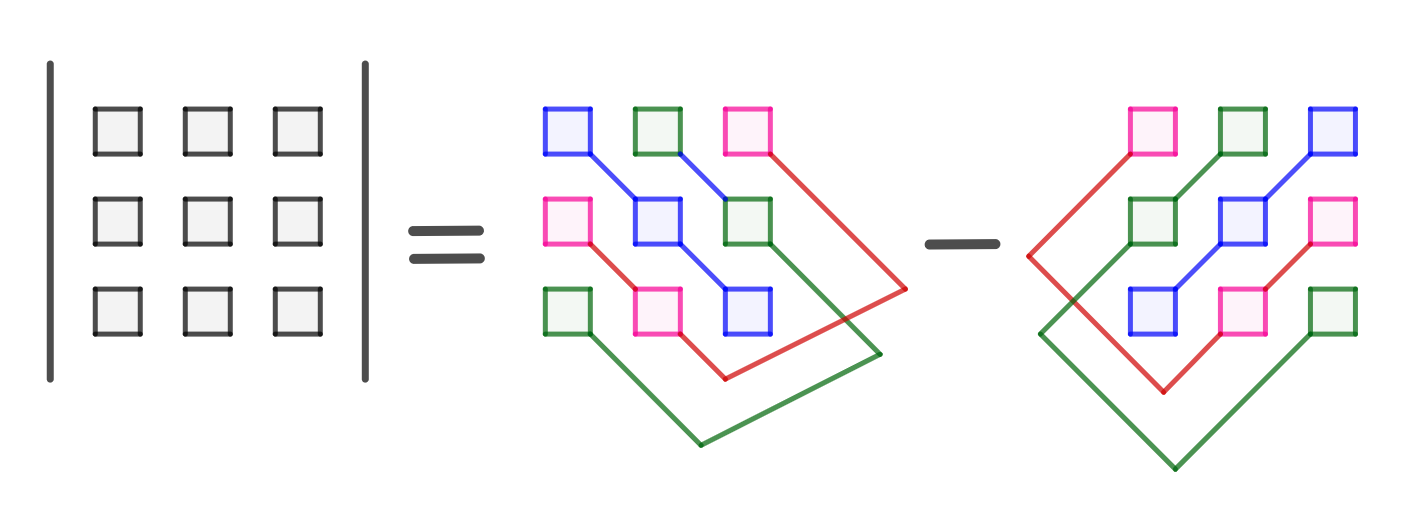
\includegraphics[width=1\textwidth]{imagenes/imagenes04/T04IM03.png}
\end{figure}

\rule{30mm}{0.1mm}

Otra regla para recordar la regla de Sarrus consiste en repetir, al final del determinante las filas $1$ y $2$ y multiplicar los elementos de las diagonales (izquierda a derecha positivas, derecha a izquierda negativas).

$|A|=\left |
\begin{array}{ccc}
a_{11} & a_{12} & a_{13} \\
a_{21} & a_{22} & a_{23} \\
a_{31} & a_{32} & a_{33}
\end{array}
\right|=
\begin{array}{ccc}
\textcolor{blue}{a_{11}} & a_{12} & a_{13} \\
\textcolor{red}{a_{21}} & \textcolor{blue}{a_{22}} & a_{23} \\
\textcolor{DarkGreen}{a_{31}} & \textcolor{red}{a_{32}} & \textcolor{blue}{a_{33}} \\
a_{11} & \textcolor{DarkGreen}{a_{12}} & \textcolor{red}{a_{13}} \\
a_{21} & a_{22} & \textcolor{DarkGreen}{a_{23}} \\
\end{array} \; - \; 
\begin{array}{ccc}
a_{11} & a_{12} & \textcolor{blue}{a_{13}} \\
a_{21} & \textcolor{blue}{a_{22}} & \textcolor{red}{a_{23}} \\
\textcolor{blue}{a_{31}} & \textcolor{red}{a_{32}} & \textcolor{DarkGreen}{a_{33}} \\
\textcolor{red}{a_{11}} & \textcolor{DarkGreen}{a_{12}} & a_{13} \\
\textcolor{DarkGreen}{a_{21}} & a_{22} & a_{23} \\
\end{array} =$

\noindent $\textcolor{blue}{a_{11}a_{22}a_{33}} + \textcolor{red}{a_{21}a_{32}a_{13}} + \textcolor{DarkGreen}{a_{31}a_{23}a_{12}} \; - \; (\textcolor{blue}{a_{13}a_{22}a_{31}} + \textcolor{red}{a_{23}a_{32}a_{11}} + \textcolor{DarkGreen}{a_{33}a_{21}a_{12})}$

Aunque es recomendable recordar la técnica anterior (mayor rapidez de cálculo mental).

\rule{30mm}{0.1mm}

\begin{ejem}
Calcula los determinantes de: 

$A=[-7/4]; \; B=\left[ \begin{array}{cc} 3&-2\\5&2  \end{array} \right]; \;  C=\left[ \begin{array}{ccc}  1 &2  &3 \\ -3&0&4 \\ 2&-1&3  \end{array} \right]$

\noindent $|A|=-7/4$

\noindent $|B|=3\cdot 2 - ((-2)\cdot 5)=6+10=16$

\noindent $|C|=1\cdot 0\cdot 3 + (-3)\cdot (-1)\cdot 3+ 2\cdot 4 \cdot 2 -(3\cdot 0 \cdot 2 + 4\cdot (-1)\cdot 1 + 3\cdot (-3)\cdot 2)=
0+9+16-(0-4-18)=25+22=47$
\end{ejem}

Para orden $4$ o superior, se recurre al desarrollo de Laplace para el cálculo de determinantes (no es válida la regla de Sarrus). Se verá en próximos apartados.

Obsérvese que para las matrices usamos paréntesis o corchetes $(a_{ij}) \text{ ó } [a_{ij}]\; $ y para los determinantes barras $|a_{ij}|$.

\section{Propiedades de los determinantes}.

Las propiedades que vamos a enunciar son válidas para determinantes de cualquier orden. Las demostraciones sobrepasan, con mucho, los objetivos de un curso de bachillerato; por lo que para cada una de ellas nos contentaremos con una mera comprobación con determinantes de ordenes $2$ o $3$, que son los que de momento, conocemos.

\begin{enumerate}[P.D. 1]
\item \colorbox{LightYellow}{$\boxed{\; |A|=|A^T|\; }$}. El determinante de una matriz coincide con el de su traspuesta.

\underline{Comprobación:}  $|A|=\left | \begin{array}{cc} 3&-2\\5&4  \end{array} \right| = 12-(-10)=22$

$|A^T|=\left | \begin{array}{cc} 3&5\\-2&4  \end{array} \right| = 12-(-10)=22$

¡ A partir de esta propiedad, todo lo que se diga para `filas' valdrá para `columnas' y viceversa !

\item Si un determinante contiene \colorbox{LightYellow}{una fila (o columna) de ceros}, el determinante es cero

\underline{Comprobación:} $|M|=\left| \begin{array}{ccc} 1&2&3\\0&0&0\\-2&3&5 \end{array} \right|= 0+0+0-(0+0+0)=0$

¡Para abreviar, en adelante, nos referiremos a `líneas' de un determinante queriendo indicar filas o columnas!

En general:

 $Det(c_1, c_2, \cdots, \textcolor{blue}{0}, \cdots , c_n)=0$, ó  $Det(f_1, f_2, \cdots, \textcolor{red}{0}, \cdots , f_n)=\textcolor{DarkGreen}{0}$
 
 Donde, con $c_1, c_2, \cdots, c_n$ queremos indicar las columnas de $M$, así como con $f_1,f_2, \cdots , f_n$ sus filas.

\item Si se \colorbox{LightYellow}{intercambian de posición dos líneas} de un determinante (dos filas o dos columnas), el determinante cambia de signo.

\underline{Comprobación:}  $\left| \begin{array}{ccc} \textcolor{blue}{1}& \textcolor{blue}{2}& \textcolor{blue}{3}\\-2&0&3\\ \textcolor{red}{-2}& \textcolor{red}{3}& \textcolor{red}{5} \end{array} \right|= 
0-18-12-(0+9-20)=-30-(-11)=-19$

 $\left| \begin{array}{ccc} \textcolor{red}{-2}& \textcolor{red}{3}& \textcolor{red}{5} \\-2&0&3\\ \textcolor{blue}{1}& \textcolor{blue}{2}& \textcolor{blue}{3}  \end{array} \right|= 
0-20+9-(0-12-18)=-11-(-30)=19$

En general: 

$Det(f_1, \cdots , \textcolor{blue}{f_i}, \cdots , \textcolor{red}{f_j} \cdots , f_n)=\textcolor{DarkGreen}- Det(f_1, \cdots , \textcolor{red}{f_j}, \cdots , \textcolor{blue}{f_i} \cdots , f_n)$

ó 

$Det(c_1, \cdots , \textcolor{blue}{c_i}, \cdots , \textcolor{red}{c_j} \cdots , c_n)=\textcolor{DarkGreen}{-} Det(c_1, \cdots , \textcolor{red}{c_j}, \cdots , \textcolor{blue}{c_i} \cdots , c_n)$

\item A una línea (fila o columna) de un determinante, si se le \colorbox{LightYellow}{añade otra} \colorbox{LightYellow}{línea} (fila o columna) del mismo determinante multiplicada por un número, el determinante no varía.

En general:

\small{$Det(f_1, \cdots , \textcolor{blue}{f_i},\cdots , f_j,  \cdots , f_n)= Det(f_1, \cdots , \textcolor{blue}{f_i}+ \textcolor{DarkGreen}{k}\cdot  \textcolor{red}{f_j}, \cdots, f_j,  \cdots , f_n)$} 

\normalsize{ó} 

\small{$Det(c_1, \cdots , \textcolor{blue}{c_i},\cdots , c_j,  \cdots , c_n)= Det(c_1, \cdots , \textcolor{blue}{c_i}+ \textcolor{DarkGreen}{k}\cdot  \textcolor{red}{c_j}, \cdots, c_j,  \cdots , c_n)$} 

\normalsize{\underline{Comprobación:}} $\left| \begin{array}{cc} 1&2\\3&4 \end{array} \right|=4-6=-2 \quad \textcolor{gris}{[\; F2 \to F2+5F1 \Rightarrow\; ]}$

$\left| \begin{array}{cc} \textcolor{blue}{1}&\textcolor{blue}{2}\\3+\textcolor{red}{5}\cdot \textcolor{blue}{1}&4+\textcolor{red}{5}\cdot \textcolor{blue}{2} \end{array} \right|=\left| \begin{array}{cc} 1&2\\8&14 \end{array} \right|=14-16=-2$

\item Si en un determinante hay una \colorbox{LightYellow}{línea igual o proporcional} a otra, el determinante es cero.

$Det(f_1, \cdots , \textcolor{blue}{f_i}, \cdots , \textcolor{red}{k} \cdot \textcolor{blue}{f_i}, \cdots , f_n)=0$

ó 

$Det(c_1, \cdots , \textcolor{blue}{c_i}, \cdots , \textcolor{red}{k}\cdot \textcolor{blue}{c_i}, \cdots , c_n)=0$

\underline{Comprobación:} 
$\; \left| \begin{array}{ccc} 1&-2&5\\-3&6&0 \\4&-8&-1 \end{array} \right|= 
-6+120+0-(120+0-6)=
\left| \begin{array}{ccc} \textcolor{blue}{1}&\textcolor{red}{-2}\cdot \textcolor{blue}{1}&5\\\textcolor{blue}{-3}&\textcolor{red}{-2} \cdot \textcolor{blue}{(-3)}&0 \\\textcolor{blue}{4}&\textcolor{red}{-2} \cdot \textcolor{blue}{4}&-1 \end{array} \right|=0$, ya que $c2=2c1$	


\item Producto de un \colorbox{LightYellow}{número por un determinante} o \colorbox{LightYellow}{`factor común'}:

$\textcolor{blue}{k}\cdot Det(f_1, \cdots , f_i, \cdots, f_j, \cdots , f_n)=
Det(f_1, \cdots , \textcolor{red}{k}\cdot f_i, \cdots, f_j, \cdots , f_n) =
Det(f_1, \cdots , f_i, \cdots, \textcolor{red}{k} \cdot f_j, \cdots , f_n)=
Det(\textcolor{red}{k} \cdot f_1, \cdots , f_i, \cdots, f_j, \cdots , f_n)= \cdots$

ó 

$\textcolor{blue}{k}\cdot Det(c_1, \cdots , c_i, \cdots, c_j, \cdots , c_n)=
Det(c_1, \cdots , \textcolor{red}{k}\cdot c_i, \cdots, c_j, \cdots , c_n) =
Det(c_1, \cdots , c_i, \cdots, \textcolor{red}{k} \cdot c_j, \cdots , c_n)=
Det(\cdot c_1, \cdots , c_i, \cdots, c_j, \cdots , \textcolor{red}{k} c_n)= \cdots$

Esta propiedad, leída de derecha a izquierda, es la '`propiedad de factor común para determinantes': si en un determinante hay una línea (fila o columna) multiplicada por un número, éste puede salir fuera del determinante multiplicando.

\underline{Comprobación:} $\textcolor{blue}{5}\cdot \left| \begin{array}{cc} 1&2\\3&4 \end{array} \right|=5\cdot (4-6)=\textcolor{blue}{5}\cdot (-2)=-10$

$\left| \begin{array}{cc} \textcolor{blue}{5}\cdot 1&\textcolor{blue}{5}\cdot 2\\3&4 \end{array} \right|=\left| \begin{array}{cc} 5&10\\3&4 \end{array} \right|=20-30=-10$

$\left| \begin{array}{cc} 1&\textcolor{blue}{5}\cdot 2\\3&\textcolor{blue}{5} \cdot 4 \end{array} \right|=\left| \begin{array}{cc} 1&10\\3&20 \end{array} \right|=20-30=-10$  

Vista como factor común: $ \left| \begin{array}{cc} 10&2\\60&8 \end{array} \right|=80-120=-40$, pero 

$ \left| \begin{array}{cc} 10&2\\60&8 \end{array} \right| =  \left| \begin{array}{cc} \textcolor{blue}{10}\cdot 1&2\\\textcolor{blue}{10} \cdot 6&8 \end{array} \right|  = \textcolor{blue}{10} \cdot  \left| \begin{array}{cc} 1&2\\6&8 \end{array} \right| = 
\textcolor{blue}{10} \cdot  \left| \begin{array}{cc} 1&2\\\textcolor{red}{2}\cdot 3&\textcolor{red}{2} \cdot 4 \end{array} \right|= \textcolor{blue}{10}\cdot \textcolor{red}{2} \cdot  \left| \begin{array}{cc} 1&2\\3&4 \end{array} \right|= \textcolor{blue}{10}\cdot \textcolor{red}{2} \cdot (4-6)=10\cdot 2\cdot (-2)=-40$

IMPORTANTE: Si $A$ es una matriz cuadrada de orden $n$ (n-filas y n-columnas), como $k\cdot A$ consiste en multiplicar por $k$ TODAS las filas (columnas) de $A$, para calcular su determinante, podemos sacar $n$-veces el número $k$ factor común de cada una de sus filas (columnas), por lo que:

\vspace{2mm} \centerline{\colorbox{LightYellow}{$\boxed{\;k\in \mathcal M_n \to det(k\cdot A)= k^n\cdot |A|\; }$}}

Nótese la diferencia de $k[A]$ y $k|A|$, el primer producto es el de un número por una matriz y el número multiplica a todos los elementos de la matriz, en el segundo caso tenemos el producto de un número por un determinante y solo se multiplica el número por una sola de sus líneas (filas o columnas).

\item Se pueden \colorbox{LightYellow}{sumar dos determinantes} de matrices del mismo tipo si las matrices son en todos sus elementos iguales excepto en una de sus líneas (fila o columna), siendo ésta la que se suma. Vista la propiedad al revés, permite descomponer un determinante como suma de otros dos en todo iguales excepto en una de sus líneas.

Generalización a determinantes de orden 3:

$\left| \begin{array}{ccc} a&b&c \\ \textcolor{blue}{x_1}&\textcolor{blue}{y_1}&\textcolor{blue}{z_1} \\ u&v&w \end{array} \right| +  
\left| \begin{array}{ccc} a&b&c \\ \textcolor{red}{x_2}&\textcolor{red}{y_2}&\textcolor{red}{z_2} \\ u&v&w \end{array} \right| =
\left| \begin{array}{ccc} a&b&c \\ \textcolor{blue}{x_1}+\textcolor{red}{x_2}&\textcolor{blue}{y_1}+\textcolor{red}{y_2}&\textcolor{blue}{z_1}+\textcolor{red}{z_2} \\ u&v&w \end{array} \right|$

\underline{Comprobación:} $\; \left| \begin{array}{cc} \textcolor{red}{4}+ \textcolor{blue}{2} \;\textcolor{gris}{(=6)}&7\\ \textcolor{red}{-3}+ \textcolor{blue}{5} \;\textcolor{gris}{(=2)}&2 \end{array} \right| =
\left| \begin{array}{cc} \textcolor{red}{4}&7\\ \textcolor{red}{-3}&2 \end{array} \right|+
\left| \begin{array}{cc} \textcolor{blue}{2} &7\\ \textcolor{blue}{5} &2 \end{array} \right|
 =$
 
 $= 12-14 = \boldsymbol{-2}= 8-(-21) \; + \; 4-(35)=29\; - \; 31 =\boldsymbol{-2} $
 
 \item El \colorbox{LightYellow}{determinante de una matriz triangular} es el producto de los elementos de la diagonal principal.
 
 En general: $\displaystyle \left| \begin{array}{cccc} a_{11} & a_{2n} & \cdots  &a_{2n}  \\ 0&a_{22}&\cdots&a_{2n}        \\0&\vdots & \ddots & \vdots \\ 0 & 0& \cdots & a_{nn} \end{array} \right| =
 a_{11} \cdot a_{22} \cdots a_{nn}=\prod_{i=1}^n a_{ii}$
 
 \underline{Comprobación:} $\left| \begin{array}{ccc}
 \textcolor{blue}{5}&\textcolor{red}0&\textcolor{red}0\\ -3&\textcolor{blue}{2}&\textcolor{red}0 \\4&-3&\textcolor{blue}{2} \end{array} \right|= \textcolor{blue}{5} \cdot \textcolor{blue}{2} \cdot \textcolor{blue}{2} +0+0-(0+0+0)=20$	
 
 \emph{Consecuencia:} \colorbox{LightYellow}{$\; \boxed {\; |I|=1\; }$}
 
 \item El determinante del producto es igual al producto de los determinantes:
 $\quad$\colorbox{LightYellow}{$\; \boxed {\; |A\cdot B|= |A| \cdot |B| \; }$}

\underline{Comprobación:} $A=\left[ \begin{array}{cc} 1&2\\3&4 \end{array} \right]; \quad B=\left[ \begin{array}{cc} 1&-1\\0&2 \end{array} \right] \to$

\noindent --- $A\cdot B= \left[ \begin{array}{cc} 1&3\\3&5 \end{array} \right] \to det(A\cdot B)= 5-9=\boldsymbol{-4}$

\noindent --- $det(A)=4-6=-2; \; det(B)=2-0=2 \to det(A) \cdot det(B)=(-2)\cdot 2=\boldsymbol{-4}$  

\item Como corolarios a la propiedad anterior: `el determinante de la potencia es la potencia del determinante' y `el determinante de la inversa es la inversa del determinante':

Como $A^n=A\cdot A \cdot \underset{\text{n-veces}}{\cdots} \cdot A $ y la propiedad anterior, deducimos que:

\vspace{2mm} \centerline{\colorbox{LightYellow}{$\; \boxed {\; |A^{n}|= |A|^n \; }$}}

 De $A\cdot A^{-1}=I; \quad |I|=1$ y la propiedad anterior, deducimos que:

\vspace{2mm} \centerline{\colorbox{LightYellow}{$\; \boxed {\; |A^{-1}|= \dfrac {1}{|A|} \; }$}}

\end{enumerate}

\normalsize{En ejercicios se verán aplicaciones las propiedades de los determinantes.}



\begin{myexampleblock}{La historia de los determinantes}

\small{Los determinantes hicieron su aparición en las matemáticas más de un siglo antes que las matrices. El término matriz fue creado por James Joseph Sylvester.}

\small{\vspace{1mm} Algunos de los más grandes matemáticos de los siglos XVIII y XIX contribuyeron al desarrollo de las propiedades de los determinantes. La mayoría de los historiadores coinciden en afirmar que la teoría de los determinantes se originó con el matemático alemán Gottfried Wilhelm Leibniz (1646-1716). Leibniz empleó los determinantes en 1693 con relación a los sistemas de ecuaciones lineales simultáneas. No obstante hay quienes creen que el matemático japonés Seki Kowa hizo lo mismo unos años antes.}

\small{\vspace{1mm} Las contribuciones más prolíficas a la teoría de los determinantes fueron las del matemático francés Agustin-Louis Cauchy (1789-1857). Cauchy escribió, en 1812 una memoria de 84 páginas que contenía la primera demostración de la fórmula $\; |A\cdot B|=|A|\cdot |B|$}

\small{\vspace{1mm} Hay algunos otros matemáticos que merecen ser mencionados aquí. El desarrollo de un determinante por cofactores fue empleado por primera vez por el matemático francés Pierre de Laplace (1749-1827).} 

\small{\vspace{1mm} Un contribuyente principal en la teoría de los determinantes fue el matemático alemán Carl Gustav Jacobi (1804-1851). Fue él con quien la palabra “determinante” ganó la aceptación definitiva.}

\rightline{\footnotesize{\emph{Fuente: Wikipedia}}\normalsize{.}}

\end{myexampleblock}



\justify


\section[Menor complementario y adjunto. Desarrollo de Laplace]{Menor complementario y adjunto. Desarrollo de Laplace}\sectionmark{Menores y adjuntos}
\sectionmark{Menores y adjuntos}


Para poder calcular determinantes de orden mayor que $3$ hemos de introducir los conceptos de `menor  complementario' y `adjunto' de un elemento de una matriz cuadrada.

\begin{defi}
Sea $A\in \mathcal M_{n\times n}$ una matriz cuadrada de orden $n$. Para cualquier elemento $a_{ij} \in A$ se define su `menor' correspondiente, y se representa por $M_{ij}$ al determinantes de orden $n-1$ que queda al eliminar de $A$ la fila$-i$ y la columna$-j$	.

Se llama `adjunto o cofactor' de $a_{ij}$ y se representa por $A_{ij}$ al menor $M_{ij}$ multiplicado por $1$ o $-1$ según sea la paridad de la suma de índices $i$ y $j$, es decir:

\centerline{\colorbox{LightYellow}{$\; \boxed{\; A_{ij}= (-1)^{i+j} \cdot M_{ij} \;}\;$}}

\end{defi}

\begin{ejem}
Sea $A=\left( \begin{matrix} 1&2&3\\4&5&6\\7&8&9 \end{matrix} \right)$. Calcula $M_{12};\; A_{12};\; M_{23};\; A_{23};\; M_{31};\; A_{31}$	

$M_{12}=\left| \begin{matrix} \cancel{1}& \boxed{\cancel{2}}&\cancel{3}\\4&\cancel{5}&6\\7&\cancel{8}&9 \end{matrix} \right|= 
\left| \begin{matrix} 4&6\\7&9 \end{matrix} \right|= 36-28=8\; $ \scriptsize{(tachamos fila 1 y columna 2)}\normalsize{.}

$A_{12}=(-1)^{1+2}\cdot M_{12}=(-1)^3\cdot 8=-8$

$M_{23}=\left| \begin{matrix} 1&2&\cancel{3}\\\cancel{4}&\cancel{5}&  \boxed{\cancel{6}} \\7&8&\cancel{9} \end{matrix} \right|=
  \left| \begin{matrix} 1&2\\7&8 \end{matrix} \right|=
  8-14=-6  $ \scriptsize{(tachamos fila 2 y columna 3)}\normalsize{.}
  
  $A_{23}=(-1)^{2+3}\cdot M_{2,3}=(-1)^5\cdot (-6)=6$
  
  $M_{31}=\left| \begin{matrix} \cancel{1}&2&3\\ \cancel{4}&5&6\\ \boxed{\cancel{7}} &\cancel{8}&\cancel{9} \end{matrix} \right|
   \left| \begin{matrix} 2&3\\5&6 \end{matrix} \right| = 12-15=-3  $
   
   $A_{31}=(-1)^{3+1}\cdot M_{31}=(-1)^4\cdot (-3)=-3$

\end{ejem}


\begin{defi}
Dada una matriz cuadrada $A$ se llama `matriz adjunta' a la que resulta de reemplazar en $A$ cada elemento $a_{ij}	$ por su correspondiente adjunto $A_{ij}$. Así, p.e., para una matriz de orden 3:

$A=\left[ \begin{matrix} a_{11}&a_{12}&a_{13}\\a_{21}&a_{22}&a_{23}\\a_{31}&a_{32}&a_{33} \end{matrix} \right] \Rightarrow  \; \; 
ad(A)=\left[ \begin{matrix} A_{11}&A_{12}&A_{13}\\A_{21}&A_{22}&A_{23}\\A_{31}&A_{32}&A_{33} \end{matrix} \right]$
\end{defi}

\begin{ejem} $A=\left[ \begin{matrix} 1&2&3 \\ 4&5&6 \\ 7&8&9 \end{matrix} \right]$, calcula su matriz adjunta.

$A_{11}=(-1)^{1+1}\; M_{11} =\left| \begin{matrix} 5&8\\8&9 \end{matrix} \right| = 45-64=-19$

$A_{12}=(-1)^{1+2}\; M_{12} =- \left| \begin{matrix} 4&6\\7&9 \end{matrix} \right| =- (36-42)=-(-6)=6$

$A_{13}=(-1)^{1+3}\; M_{13} =\left| \begin{matrix} 4&5\\7&8 \end{matrix} \right| = 32-35=-3$

$A_{21}=(-1)^{2+1}\; M_{21} =-\left| \begin{matrix} 2&3\\8&9 \end{matrix} \right| = -(18-24)=-(-6)=6$

$A_{22}=(-1)^{2+2}\; M_{22} =\left| \begin{matrix} 1&3\\7&9 \end{matrix} \right| = 9-21=-12$

$A_{23}=(-1)^{2+3}\; M_{23} =-\left| \begin{matrix} 1&2\\7&8 \end{matrix} \right| = -(8-14)=-(-6)=6$

$A_{31}=(-1)^{3+1}\; M_{31} =\left| \begin{matrix} 2&3\\5&6 \end{matrix} \right| = 12-15=-3$

$A_{32}=(-1)^{3+2}\; M_{32} =- \left| \begin{matrix} 1&3\\4&6 \end{matrix} \right| = -(6-12)=-(-6)=6$

$A_{33}=(-1)^{3+3}\; M_{33} =\left| \begin{matrix} 1&2\\4&5 \end{matrix} \right| = 5-8=-3$

Luego: $\; \; ad(A)=\left[ \begin{matrix} -19&6&-3\\6&-12&6\\-3&6&-3\end{matrix} \right]$

\end{ejem}


El siguiente teorema, que daremos sin demostración, permite calcular el determinante de cualquier matriz cuadrada de orden $n$ \textcolor{gris}{($\forall n \in \mathbb N$)} en función, eso sí, de $n$ determinantes de orden $n-1$. Se trata del `desarrollo de Laplace'.

\begin{teor}{Desarrollo de Laplace de un determinante.}
	
	El determinante de una matriz se puede desarrollar como suma de los productos de los elementos de una línea (fila o columna) cualquiera por sus correspondientes adjuntos.
	
	Sea $A=\left[
\begin{matrix}
a_{11} & a_{12} & \cdots & a_{1j} & \cdots & a_{1n} \\
a_{21} & a_{22} & \cdots & a_{2j} & \cdots & a_{2n} \\
a_{31} & a_{32} & \cdots & a_{3j} & \cdots & a_{3n} \\
\vdots & \vdots & \ddots & \vdots & \ddots & \vdots \\
a_{i1} & a_{i2} & \cdots & a_{ij} & \cdots & a_{in} \\
\vdots & \vdots & \ddots & \vdots & \ddots & \vdots \\
a_{m1} & a_{m2} & \cdots & a_{mj} & \cdots & a_{mn} \\
\end{matrix}
\right] \Rightarrow$

\vspace{3mm} $|A|=a_{11}A_{11}+a_{12}A_{12}+\cdots +a_{1n}A_{1n} \text{ (desarrollo primera fila) }= $

$=a_{13}A_{13}+a_{23}A_{23}+\cdots +a_{n3}A_{n3} \text{ (desarrollo tercera columna) } = $

$=a_{1j}A_{1j}+a_{2j}A_{2j}+\cdots +a_{nj}A_{nj} \text{ desarrollo columna-j )}= \displaystyle \sum_{k=1}^n a_{kj}A_{kj} =$

$=a_{i1}A_{i1}+a_{i2}A_{i2}+\cdots +a_{in}A_{in} \text{ (desarrollo fila-i) } = \displaystyle \sum_{k=1}^n a_{ik}A_{ik}=etc$
	
\end{teor}

\begin{ejem} Usando el desarrollo de Laplace:

Calcula: $a)\;  \left| \begin{matrix} 1&2&3\\4&5&6\\7&8&9 \end{matrix} \right|; \quad b)\; 
\left| \begin{matrix} 1&0&3&-1\\0&2&-1&-2\\2&0&5&2 \\ 0&0&-3&1  \end{matrix} \right|\quad c)\; \left| \begin{matrix} 1&5\\-3&3 \end{matrix} \right|$ 

----- Cálculo del $|A|$ :

* por adjuntos de la tercera columna:

$|A|= 
3\cdot (-1)^{3+1}\cdot \left| \begin{matrix} 4&5 \\ 7&8 \end{matrix} \right|	+
6\cdot (-1)^{3+2}\cdot \left| \begin{matrix} 1&2 \\ 7&8 \end{matrix} \right|+
9\cdot (-1)^{3+3}\cdot \left| \begin{matrix} 1&2 \\ 4&5 \end{matrix} \right|
=
3\cdot (+1) \cdot (32-35) + 6\cdot (-1) (8-14) + 9 \cdot (+1) \cdot (5-8)=
-9 +36 -27=0$

* por adjuntos de la segunda fila:

$|A|=4\cdot (-1)^{2+1}\left| \begin{matrix} 2&3\\8&9  \end{matrix} \right| +
5\cdot (-1)^{2+2}\cdot \left| \begin{matrix} 1&3\\7&9  \end{matrix} \right|+
6\cdot (-1)^{2+3}\cdot \left| \begin{matrix} 1&2\\7&8  \end{matrix} \right|=
 4\cdot (-1) \cdot (18-24) + 5\cdot (+1)\cdot (9-21) + 6 \cdot (-1) (8-14)=
 24-60+36 =0 $
 
 * por Sarrus, evidentemente, también dará cero:
 
 $A= 45+96+84-(105+48+72)=225-225=0$
 
 ----- Cálculo del $|B|$:
 
 * por adjuntos de la tercera fila:

$|B|= 2\cdot (-1)^{3+1}\; \left| \begin{matrix} 0&3&-1\\2&-1&2\\0&-3&1  \end{matrix} \right| +
\cancelto{0}{\boldsymbol{0} \cdot (-1)^{3+2} \; \left| \begin{matrix}  1&3&-1\\0&-1&2\\0&-3&1 \end{matrix} \right|} +$

$+5 \cdot (-1)^{3+3}\; \left| \begin{matrix}  1&0&-1\\0&2&2\\0&0&1 \end{matrix} \right|+ 
2 \cdot (-1)^{3+4} \; \left| \begin{matrix} 1&0&3\\0&2&-1\\0&0&-3   \end{matrix} \right|= $

$=2\cdot(+1) \cdot (0+6+0-(0+0+6)) +0+$

$+5\cdot(+1)\cdot (2+0+0-(0+0+0)) + 2\cdot (-1) \cdot (-6+0+0-(0+0+0))=$

$=0 \; + \; 0 \; + \; 10 \; + \; 12 = \; \boldsymbol{22} $

\scriptsize{Los dos últimos Sarrus son determinantes de matrices triangulares, luego son iguales al producto de los elementos de la diagonal principal, con lo que se ahorra tiempo de cálculo}\normalsize{.}

Nótese que, como `estrategia', es conveniente hacer el desarrollo de Laplace por los elementos de la línea que contenga más ceros, lo que hará que tengamos que calcular menos determinantes, por ello:

* por adjuntos de la segunda columna:

$|B|=  0\; + \; 2 \cdot (1-)^{2+2} \cdot \left| \begin{matrix} 1&3&-1\\2&5&2\\0&-3&1  \end{matrix} \right|\; + 0 \; + \; 0=$

$=2\cdot (5+6+0-(0-6+6))= 2 \cdot 11 = \boldsymbol {22}$


----- Cálculo de $|C|$:

* por adjunto segunda columna:

$|C|= 5 \cdot (-1)^{1+2} |-3|+ 3\cdot (-1)^{2+2}\cdot |1|= 5(-1)(-3)+3\cdot 1\cdot 1=15+3=\boldsymbol{18}$

* por adjuntos de la primera fila:

$|C|= 1\cdot (-1)^{1+1}\;|3|+5\cdot (-1)^{1+2}\; |-3| = 3+15=\boldsymbol{18}$

* por la definición:  $|C|=3-(-15)=\boldsymbol{18}$
 
\end{ejem}

\vspace{-4mm}%****************************
\subsection{Método Chio}
\vspace{-2mm}%****************************

\begin{myblock}{Método Chio}
\begin{multicols}{2}
\small{Utilizando las propiedades de los determinantes se trata de hacer ceros en todos los elementos de una línea excepto uno de ellos, para luego desarrollarlo por los adjuntos de esa línea}\normalsize{}.

\begin{figure}[H]
	\centering
	
\includegraphics[width=0.3\textwidth]{imagenes/imagenes04/T04IM01.png}
\end{figure}
\end{multicols}
\end{myblock}

\vspace{4mm}
\begin{ejem}
Calcula:  $\left|
\begin{matrix}
1&2&3&4\\-1& \boldsymbol{0}&1&2\\2&\boldsymbol{0}&1&1\\2&2&-2&3&	
\end{matrix}    
\right|=\; [F4 \to F4-F1]\; =$	

$\left|
\begin{matrix}
1&2&3&4\\-1&\boldsymbol{0}&1&2\\2&\boldsymbol{0}&1&1\\1&\boldsymbol{0}&-5&1&	
\end{matrix}    
\right|= 2 \; (-1)^{1+2} \; \left|
\begin{matrix}
-1&1&2\\2&1&1\\1&-5&-1
\end{matrix}    
\right|= \text{ (Sarrus) }=$

$ = 2\; (-1)\; (-23) = \boldsymbol{46}$

\vspace{4mm}
\underline{Observación 1}: No confundir las propiedades de los determinantes por las transformaciones de Gauss: Gauss permite cambiar una fila por un número ($\neq 0$) multiplicada por ella más un número por otra; en los determinantes se puede cambiar una fila (o columna) por `ella misma' (multiplicada por `+1') más un número por otra fila (o columna). \underline{La línea a cambiar} \underline{en un determinante no puede estar multiplicada por ningún número distinto} \underline{ de la unidad positiva} (ni siquiera se puede tomar para restar)  

\footnotesize{\textcolor{gris}{$\begin{array}{lll} *\; \* Fi \to Fi-3Fj \quad \text{Bién} \\
 *\; \* Fi \to 3Fj-Fi \quad \text{Mal: }\; (-1)\cdot Fi \\
  *\; \* Fi \to 2Fi+3Fj \quad \text{Mal: }\; 2\cdot Fi \end{array}$}}\normalsize{.}

\underline{Observación 2}: Hay una gran diferencie entre el producto de un número por una matriz $k\cdot(A)$, en que se multiplican TODOS los elementos de la matriz por $k$ y el producto de un número por un determinantes, $k\cdot |A|$, que consiste en elegir UNA SOLA LÍNEA de $A$ (fila o columna) y multiplicar sus elementos por $k$ (recuérdese lo dicho en la propiedad P.D. 6 de determinantes).

\underline{Observación 3}: Para buscar `ceros' en una columna, combinamos filas. Para buscar `ceros' en una fila, combinamos columnas (Ver en problemas resueltos).

\end{ejem}


\vspace{10mm}
\begin{myexampleblock}{Aplicaciones geométricas de los determinantes}

%\vspace{10mm}
\begin{figure}[H]
	\centering
	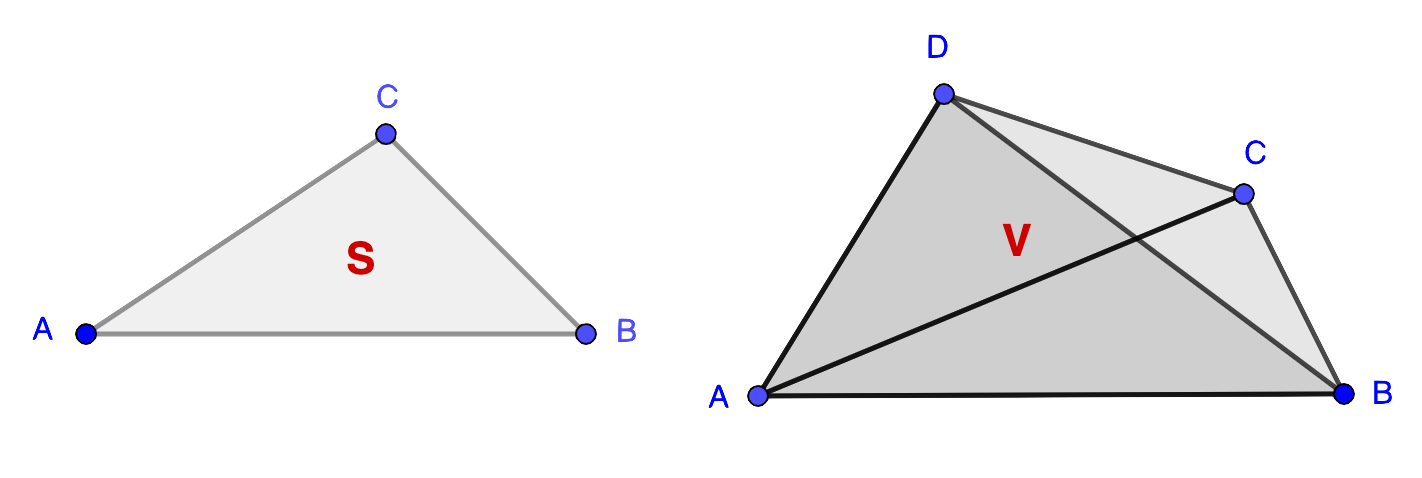
\includegraphics[width=1\textwidth]{imagenes/imagenes04/T04IM04.png}
\end{figure}

Área del triángulo de vértices $A(x_1,y_1),\; B(x_2,y_2),\; C(x_3,y_3)$

Sea $\Delta = \left| \begin{matrix} x_1&x_2&x_3 \\ y_1&y_2&y_3\\1&1&1 \end{matrix} \right|$, entonces, 

Área $S_{ABC}= \dfrac 1 2 \; abs \; \Delta = \dfrac 1 2 \;|\Delta|$ (la mitad del valor absoluto del determinante $\Delta$).

Volumen de un tetraedro de vértices  $A(x_1,y_1,z_1),\; B(x_2,y_2,z_2),$

\noindent $C(x_3,y_3,z_3), \; D(x_4,y_4,z_4)$.

\centerline{Vol. $V=\dfrac 1 6\; abs\; \left( \left| \begin{matrix} x_1&y_1&z_1&1 \\   x_2&y_2&z_2&1  \\  x_3&y_3&z_3&1  \\  x_4&y_4&z_4&1  \end{matrix} \right| \right)$}

\end{myexampleblock}



\justify




\section{Inversa de una matriz por adjuntos}

Ea ahora cuando vamos a desarrollar un método más potente que el de Gauss para el cálculo de la inversa de una matriz cuadrada. Además, este método nos dice si dada una matriz cuadrada cualquiera tiene inversa. (Lo exponemos como un teorema sin demostración).

\begin{teor}{Inversa por adjuntos.}

$\forall A\in \mathcal M_{n \times n}(\mathbb R): \; \exists A^{-1} \Leftrightarrow |A|\neq 0 \; \text{ además }	\;$ \colorbox{LightYellow}{$\boxed{\; A^{-1}=\dfrac 1 {|A|}\; ad(A^T)\; }$}

La inversa de una matriz es uno partido por su determinante \textcolor{gris}{(claro, si el determinantes es cero, no hay inversa)} de la matriz adjunta de la matriz traspuesta. --Puesto que las operaciones de trasposición y adjunto conmutan (se puede comprobar, hágase) algunos autores hablan de la traspuesta de la matriz adjunta-- $[\;ad(A^T)=(ad A)^T \;]$.
\end{teor}

\begin{defi}
Dada $A\in \mathcal M_{n}:$

si $|A|=0 \to \nexists A^{-1} \Rightarrow $ se dice que $A$ es `singular'.

si $|A|\neq 0 \to \exists A^{-1} \Rightarrow $ se dice que $A$ es `regular o invertible'.
\end{defi}


\begin{ejem}
	En el tema anterior, en el apartado de calculo de inversas de matrices por Gauss, vimos:
	
	$B=\left[\begin{matrix} 1&0&2\\3&1&-1\\-2&1&5  \end{matrix}\right] \to B^{-1}=
\dfrac 1 {16} \left[ \begin{matrix} 6&2&-2 \\ -13&9&7 \\5&-1&1  \end{matrix} \right]$

Comprobemos que obtenemos el mismo resultado por el método de los adjuntos:  $B^{-1}=\dfrac 1 {|B|}\; ad(B^T)$:

El \underline{primer caso} es calcular $|B|$, puesto que si es $0$ la matriz será singular o no invertible y habríamos acabado.

Por Sarrus: $|B|=5+6+0-(-4-1+0)=11-(-5)=16\neq 0 \to \exists B^{-1}$

El \underline{segundo paso} es calcular la traspuesta de $B$, no se nos vaya a olvidar \textcolor{gris}{(se puede calcular después del cálculo de la matriz adjunta, como hemos dicho anteriormente, puesto que trasposición y adjunto son operaciones que conmutan)}

$B^T=\left[\begin{matrix} 1&3&-2\\0&1&1\\2&-1&5  \end{matrix}\right]$. Como \underline{tercer paso}, vamos a calcular $ad(B^T)$


$B^T_{11}= (-1)^{1+1}\; \left| \begin{matrix} 1&1\\-1&5 \end{matrix} \right|=
(5-(-1))=6$

$B^T_{12}= (-1)^{1+2}\; \left| \begin{matrix} 0&1\\2&5 \end{matrix} \right|=
-(0-(2))=2$

$B^T_{13}= (-1)^{1+3}\; \left| \begin{matrix} 0&1\\2&-1 \end{matrix} \right|=
(0-(2))=-2$



$B^T_{21}= (-1)^{2+1}\; \left| \begin{matrix} 3&-2\\-1&5 \end{matrix} \right|=
-(15-(2))=-13$

$B^T_{22}= (-1)^{2+2}\; \left| \begin{matrix} 1&-2\\2&5 \end{matrix} \right|=
(5-(-4))=9$

$B^T_{23}= (-1)^{2+3}\; \left| \begin{matrix} 1&3\\2&-1 \end{matrix} \right|=
-(-1-(6))=7$


$B^T_{31}= (-1)^{3+1}\; \left| \begin{matrix} 3&-2\\1&1 \end{matrix} \right|=
(3-(-2))=5$

$B^T_{32}= (-1)^{3+2}\; \left| \begin{matrix} 1&-2\\0&1 \end{matrix} \right|=
-(1-(0))=-1$

$B^T_{33}= (-1)^{3+3}\; \left| \begin{matrix} 1&3\\0&1 \end{matrix} \right|=
(1-(0))=1$

Por lo que $B^{-1}=
\dfrac 1 {16} \left[ \begin{matrix} 6&2&-2 \\ -13&9&7 \\5&-1&1  \end{matrix} \right]$, que coincide con la calculada por el método de Gauss, como era de esperar.

\end{ejem}

\underline{Nota}: Hemos llamado $A$ a una matriz (cuadrada), $a_{ij}$ a sus elementos; $M_{ij}$ a sus menores y $A_{ij}$ a sus adjuntos. El problema surge cuando hablemos de matrices $M$. Proponemos la solución de que $m_{ij}$ sean sus elementos, $M_{ij}$ los menores, entonces a los adjuntos les llamaremos $\boldsymbol{M}_{ij}$ ó $ad_{ij}$.

\begin{figure}[]
	\centering
	
\includegraphics[width=0.8\textwidth]{imagenes/imagenes04/T04IM02.png}
\end{figure}

\begin{teor}{Propiedades de la matiz inversa}

Recordemos las propiedades de la matriz inversa vistas en el capítulo anterior:

Definición:  $AA^{-1}=A^{-1}A=I\quad $
Cálculo: $A^{-1}=\dfrac 1 {|A|}\; ad(A^T)$

\begin{multicols}{2}
\begin{enumerate}
\item $(A^{-1})^{-1}=A$
\item $(k\cdot A)^{-1}= \dfrac 1 k \; A^{-1}$
\item $(A\cdot B)^{-1}=B^{-1} \cdot A^{-1}$
\item $(A^T)^{-1}=(A^{-1})^T$
\end{enumerate}
\end{multicols}
\end{teor}

\subsection{Ecuaciones matriciales}

Son ecuaciones y sistemas en que las incógnitas (y quizás también los coeficientes) son matrices. $X,\; Y, \; \cdots $ son matrices incógnita, $A,\; B, \; C, \; \cdots $ son datos (matrices).

Este tipo de ejercicios constará usualmente  de dos partes: despejar teóricamente la incógnita (si es posible) y realizar las operaciones indicadas a que se ha llegado al despejar.

--- * Sistemas de ecuaciones matriciales lineales:

$\begin{cases} aX+bY=M\\cX+dY=N \end{cases}$, con $a,b,c,d \in \mathbb R$, coeficientes reales y $X,Y,M,N \in \mathcal M (\mathbb R)$, siendo $X$ e $Y$ las matrices incógnita y $M$ y $N$ matrices conocidas (datos).

Se resuelven, teóricamente, como si se tratase de sistemas de ecuaciones lineales cualesquiera y, es después, cuando se realizan las operaciones matriciales necesarias para la solución del sistema.

\begin{ejem} Resuelve $\begin{cases} X-2Y=\left( \begin{matrix}  1&0\\1&1 \end{matrix} \right) \\ X+3Y=\left( \begin{matrix}  0&2\\4&-3 \end{matrix} \right) \end{cases}$ 

Si a la segunda ecuación le restamos la primera: 

$\boldsymbol{Y}=\left( \begin{matrix}  0&2\\4&-3 \end{matrix} \right) -\left( \begin{matrix}  1&0\\1&1 \end{matrix} \right)=\boldsymbol{ \left( \begin{matrix} -1&2 \\3&-4  \end{matrix}  \right)}$

Sustituyendo en la primera ecuación:
$\boldsymbol{ X}=\left( \begin{matrix}  1&0\\1&1 \end{matrix} \right)+2Y=$

$=\left( \begin{matrix}  1&0\\1&1 \end{matrix} \right)+2\left( \begin{matrix} -1&2 \\3&-4  \end{matrix}  \right)=
\left( \begin{matrix}  1&0\\1&1 \end{matrix} \right)
+\left( \begin{matrix} -2&4 \\6&-8  \end{matrix}  \right)=
\boldsymbol{ \left( \begin{matrix}  -1&4\\7&-7 \end{matrix} \right)}$

\end{ejem}

--- * Ecuaciones matriciales: 

Son ecuaciones en que tanto coeficientes como incógnitas son matrices.

$AX=B \to \text{ si } \exists A^{-1} \; \therefore \; $ `premultiplicando por $A^{-1}$:

$A^{-1}(AX)= A^{-1}(B) \to A^{-1}AX=IX=\boldsymbol{A=A^{-1}B}$

Solo quedaría, en un problema usual, hacer las operaciones que han aparecido al despejar. En este caso, calcular la inversa de $A$ y `premultiplicar' por $B$ 

\underline{¡Ojo!}: el orden en que se multiplican matrices es MUY importante, por eso insistimos en lo de `premultiplicar' y `postmultiplicar' 

Veamos otros ejemplos teóricos de resolución de ecuaciones matriciales:

\noindent * $XM=N \to$

Si $\exists M^{-1}$, postmultiplicando: $XMM^{-1}=XI=\boldsymbol{X=NM^{-1}}$

\noindent * $AXB=C \to $

Si existen $A^{-1}$ y $B^{-1}$, premultiplicando por $A^{-1}$ y postmultiplicando por $B^{-1}$ (lo hacemos más explícitamente en este caso):

$\textcolor{red}{A^{-1}} \cdot \textcolor{blue}{AXB}  \cdot \textcolor{red}{B^{-1}}= $
$\textcolor{red}{A^{-1}} \cdot \textcolor{blue}{C} \cdot \textcolor{red}{B^{-1}} $
$\to A^{-1}AXBB^{-1}=A^{-1}CB^{-1} \to $

$IXI=A^{-1}CB^{-1} \Rightarrow X=A^{-1}CB^{-1}$

\noindent * $ABX=C \to $

Si existen $A^{-1}$ y $B^{-1}$, premultiplicando por $A^{-1}$ y luego por $B^{-1}$:

$ \textcolor{red}{A^{-1}} ABX = \textcolor{red}{A^{-1}} C \to  A^{-1}ABX=A^{-1}C\to IBX=A^{-1}C \Rightarrow$ 

$BX=A^{-1}C$. Ahora por $B^{-1}\; $: $\textcolor{blue}{B^{-1}}BX=\textcolor{blue}{B^{-1}}A^{-1}C \to $

$BB^{-1}X=B^{-1}A^{-1}C \to IX=B^{-1}A^{-1}C  \Rightarrow X=B^{-1}A^{-1}C $

Obsérvese que también podíamos haber hecho: $(AB)X=C$, si existe $(AB)^{-1} \to (AB)^{-1}(AB)X=(AB)^{-1}C \to IX=(AB)^{-1}C \qquad  \Rightarrow \qquad X=(AB)^{-1}C$, que evidentemente es el mismo resultado anterior, puesto que $(AB)^{-1}=B^{-1}A^{-1}$

\noindent * $AX=BX+C \to$ 

Primero aislemos la matriz incógnita $X$ en un solo miembro de la ecuación:

$AX-BX=C \to (A-B)X=C \to \text{ si } \; \exists (A-B)^{-1} \quad  \therefore \; $

$(A-B)^{-1}(A-B)X=(A-B)^{-1}C \to IX=(A-B)^{-1}C \Rightarrow $

$X=(A-B)^{-1}C$

\noindent * $XM=NX+P \to$ 

Como en el caso anterior: $XM-NX=P$, sacando `factor común por la izquierda':

$X(M-N)=P$, si existe $(M-N)^{-1}$, postmultiplicando en ste caso:

$X(M-N)(M-N)^{-1}=P(M-N)^{-1} \to XI=P(M-N)^{-1} \Rightarrow $

$X=P(M-N)^{-1}$

\noindent * $XM=2X+N$

Análogamente al caso anterior: $XM-2X=N \to X(M-2)= \cdots $ ¡Un momento!: $M-2$ no tiene ningún sentido. ASTUCIA: usemos la matriz $I$:

\small{$XM-2X=N \to XM-X2=N \to XM-X2\textcolor{red}{I}=N \to X(M-2I)=N$}\normalsize{.}

Si existe la inversa de la matriz $M-2I$, que ahora sí tiene sentido, postmultiplicando tendremos:

$X(M-2I)(M-2I)^{-1}=N(M-2I)^{-1} \to XI=N(M-2I)^{-1} \Rightarrow $

$X=N(M-2I)^{-1}$

\noindent * etc.  En problemas veremos, y resolveremos, más casos.





\subsection{Forma matricial de un SEL}

Un sistema de ecuaciones lineales `cuadrado', es decir, con tantas ecuaciones como incógnitas, se puede interpretar como una ecuación matricial:

$\begin{cases} a_{11}x_1+a_{12}x_2 + \cdots + a_{1n}x_n &=b_1 \\
a_{12}x_1+a_{22}x_2 + \cdots + a_{2n}x_n &=b_2 \\
\cdots + \cdots + \cdots + \cdots + \cdots  &=\cdots \\
a_{n1}x_1+a_{n2}x_2+\cdots +a_{nn}x_n &=b_n  \end{cases} \quad \Leftrightarrow \quad \boxed{\; AX=B\; \; }$	,

donde:
$A=\left( \begin{matrix}  a_{11}&a_{12}& \cdots &a_{1n} \\
a_{12} &a_{22} &\cdots &a_{2n} \\
\cdots & \cdots & \cdots & \cdots  \\
a_{n1} &a_{n2} &\cdots &a_{nn}    \end{matrix} \right); \; X=\left( \begin{matrix} x_1\\x_2\\ \vdots \\x_n \end{matrix} \right); \; B=\left( \begin{matrix} b_1\\b_2\\ \vdots \\b_n \end{matrix} \right)$

$A$ es la matriz de los coeficientes, $X$ la de incógnitas y $B$ la de términos independientes.

Es decir: 

\noindent \colorbox{LightYellow}{\scriptsize{$\boxed{\begin{cases} a_{11}x_1+a_{12}x_2 + \cdots + a_{1n}x_n &=b_1 \\
a_{12}x_1+a_{22}x_2 + \cdots + a_{2n}x_n &=b_2 \\
\cdots + \cdots + \cdots + \cdots + \cdots  &=\cdots \\
a_{n1}x_1+a_{n2}x_2+\cdots +a_{nn}x_n &=b_n  \end{cases}  \Leftrightarrow 
\left( \begin{matrix}  a_{11}&a_{12}& \cdots &a_{1n} \\
a_{12} &a_{22} &\cdots &a_{2n} \\
\cdots & \cdots & \cdots & \cdots  \\
a_{n1} &a_{n2} &\cdots &a_{nn}    \end{matrix} \right) \cdot \left( \begin{matrix} x_1\\x_2\\ \vdots \\x_n \end{matrix} \right)=\left( \begin{matrix} b_1\\b_2\\ \vdots \\b_n \end{matrix} \right)}$}}

\normalsize{En} el caso de que $\exists A^{-1}$, se puede resolver la ecuación matricialemente.

Consideraciones: para usar este método es necesario que el sistema sea cuadrado y la matriz de los coeficientes sea distinta de cero (para que $\exists A^{-1}$. Además, el cálculo de una inversa suele ser largo. El método de Gauss sirve para cualquier sistema de ecuaciones.

En el apartado de problemas veremos como resolver matricialmente un SEL.



\section{Ejercicios}

\subsection{Ejercicios resueltos}

%Cálculo Sarrus-Laplace

\begin{ejre} Calcula:

\noindent \small{$a)\; \left| \begin{matrix} 2&-1\\8&5  \end{matrix} \right| \; \;    
b)\; \left| \begin{matrix} -2&1&3\\5&-1&0\\0&2&-6  \end{matrix} \right| \; \; 
c)\; \left| \begin{matrix} 2&1&0&-1\\3&1&2&-1\\2&-1&1&0\\0&1&1&2  \end{matrix} \right| \; \; 
d)\; \left| \begin{matrix} 1&-1&0&2&0\\1&0&2&0&0\\0&0&-1&2&3\\-1&2&2&-1&0\\2&5&0&1&-2   \end{matrix} \right| \; \; $}

\end{ejre}

\begin{proofw}\renewcommand{\qedsymbol}{$\diamond$}

\normalsize{-----} a) $\left| \begin{matrix} 2&-1\\8&5  \end{matrix} \right|=10-(-8)=\boldsymbol{ 18}$	

\noindent ----- b) $\left| \begin{matrix} -2&1&3\\5&-1&0\\0&2&-6  \end{matrix} \right|= -12+30+0-(0+0-30)=\boldsymbol{48}$


\noindent ----- c) $\left| \begin{matrix} 2&1&0&-1\\3&1&2&-1\\2&-1&1&0\\0&1&1&2  \end{matrix} \right| = \left[ \begin{matrix} F2 \to F2-2F4\\ F3 \to F3-F4 \end{matrix} \right] = \left| \begin{matrix} 2&1&\boxed{0}&-1\\3&-1&\boxed{0}&-5\\2&-2&\boxed{0}&-2\\0&1&1&2  \end{matrix} \right| =\to $

Desarrollamos por Laplace por los adjuntos de la tercera columna:

\noindent $\to = 0\; +\; 0\; +\; 0\; +\; 1\cdot (-1)^{4+3} \left| \begin{matrix} 2&1&-1\\3&-1&-5\\2&-2&-2 \end{matrix} \right| = - [\; 4+6-10-(2+20-6) \; ]= -[0-(16)]=\boldsymbol{ 16} $

\noindent ----- d) $ \left| \begin{matrix} 1&-1&0&2&\boldsymbol{0}\\1&0&2&0&\boldsymbol{0}\\0&0&-1&2&3\\-1&2&2&-1&\boldsymbol{0}\\2&5&0&1&-2   \end{matrix} \right| =  \dfrac {\colorbox{Yellow}{3}} {3}  \left| \begin{matrix} 1&-1&0&2&\boldsymbol{0}\\1&0&2&0&\boldsymbol{0}\\0&0&-1&2&3\\-1&2&2&-1&\boldsymbol{0}\\\colorbox{Yellow}{2}&\colorbox{Yellow}{5}&\colorbox{Yellow}{0}&\colorbox{Yellow}{1}&\colorbox{Yellow}{-2}   \end{matrix} \right|= \to  $

Multiplicamos, y dividimos, la última fila por $3$, para tenerla preparada y buscar `ceros en la quinta columna): \textcolor{gris}{(también hubiésemos podido buscar `ceros' en la segunda fila, donde ya hay $3$, cambiando $C2$ por$C2-2C1$)}

\noindent $\dfrac 1 3  \left| \begin{matrix} 1&-1&0&2&\boldsymbol{0}\\1&0&2&0&\boldsymbol{0}\\0&0&-1&2&3\\-1&2&2&-1&\boldsymbol{0}\\\colorbox{Yellow}{6}&\colorbox{Yellow}{15}&\colorbox{Yellow}{0}&\colorbox{Yellow}{3}&\colorbox{Yellow}{-6}   \end{matrix} \right|= 
[\;F5 \to F5+2F3\;] = \to $

\noindent $\dfrac 1 3  \left| \begin{matrix} 1&-1&0&2&\text{\textst{ 0 }}	\\1&0&2&0&\text{\textst{ 0 }}	\\\text{\textst{ 0 }}	&\text{\textst{ 0 }}	&\text{\textst{ -1 }}	&\text{\textst{ 2 }}	&\text{\textst{ 3 }}	\\-1&2&2&-1&\text{\textst{ 0 }}	\\6&15&-2&7&\text{\textst{ 0 }}	   \end{matrix} \right|= $ (Laplace $5^a$ columna) $=\to$

\noindent $\to =0\; +\; 0\; + \dfrac 1 3\; 3 \cdot (-1)^{3+5} \left|
\begin{matrix}   1&-1&0&2\\1&\boldsymbol{ 0}&2&\boldsymbol{ 0}\\-1&2&2&-1 \\6&15&-2&7  \end{matrix} \right| = [\; C3 \to C3-2C1 \;  ] = \to $

\noindent $=+\left|
\begin{matrix}   1&-1&-2&2\\1&\boldsymbol{ 0}&\boldsymbol{0} &\boldsymbol{ 0}\\-1&2&4&-1 \\6&15&-14&7  \end{matrix} \right|=$  (Lapalace $2^a$ fila) 
$=   \left|
\begin{matrix}   \text{\textst{ 1 }}&-1&-2&2\\\text{\textst{ 1 }}&\text{\textst{ 0 }}&\text{\textst{ 0 }} &\text{\textst{ 0 }}\\\text{\textst{ 1 }}&2&4&-1 \\\text{\textst{ 6 }}&15&-14&7  \end{matrix} \right| = $


\noindent $1\cdot (-1)^{2+1}\; \left| \begin{matrix}  -1&-2&2\\2&4&-1\\15&-14&7 \end{matrix} \right| +0+0+0= -[-28-56+30-(120-14-28)]=-[-54-(78)]-[-132]=\boldsymbol{132}$
\end{proofw}


\begin{ejre}
Dada $A=\left[ \begin{matrix}2&3&0\\0&1&2\\-1&0&2 \end{matrix} \right]\;$, calcula los siguientes adjuntos: $A_{23}; \; A_{32}; \; A_{11}$
\end{ejre}

\begin{proofw}\renewcommand{\qedsymbol}{$\diamond$}

$A_{23}=(-1)^{2+3}\;M_{23}= (-1)\; \left| \begin{matrix} 2&3\\-1&0
 \end{matrix} \right|= (-1)\; (0-(-3)) = \boldsymbol{-3}$
 
\noindent $A_{32}=(-1)^{3+3}\;M_{32}= (-1)\; \left| \begin{matrix} 2&0\\0&2
 \end{matrix} \right|= (-1)\; (4-(0)) = \boldsymbol{-4}$	
 
\noindent $A_{11}=(-1)^{1+1}\;M_{1}= +\; \left| \begin{matrix} 1&2\\0&2
 \end{matrix} \right|=  (2-(0)) = \boldsymbol{2}$
\end{proofw}

\begin{ejre}
	Sea $\; A_n=\left( \begin{matrix}
 1&1&1&\cdots&1 \\ -1&2&1&\cdots &1	\\ -1&-1&2&\cdots &1 \\ \vdots & \vdots & \vdots & \ddots & \vdots \\-1&-1&-1& \cdots &2
 \end{matrix} \right)\; $. 
 
 Calcula $det(A_2); \; det(A_3); \; det(A_4)$. ¿Qué valdrá el $\; det(A_n)\; $?

\end{ejre}

\begin{proofw}\renewcommand{\qedsymbol}{$\diamond$}
	$A_2= \left| \begin{matrix} 1&1\\-1&2   \end{matrix} \right|=2-(-1)=3=3^{2-1}$
	
\noindent $A_2= \left| \begin{matrix} 1&1&1\\-1&2&1 \\ -1&-1&2   \end{matrix} \right|=4+1-1 -(-2-1-2) =4-(-5)=9=3^2=3^{3-1}$

\noindent $A_3= \left| \begin{matrix} 1&1&1&1\\-1&2&1&1 \\ -1&-1&2&1 \\ -1&-1&-1&2   \end{matrix} \right|= \textcolor{gris}{\begin{cases} F2\to F1+F1 \\ F3\to F3+F1  \\ F4\to F4+F1  \end{cases}} = 
\left| \begin{matrix} 1&1&1&1\\0&3&2&2 \\ 0&0&3&2 \\ 0&0&0&3   \end{matrix} \right| = \textcolor{gris}{diagonal}= 1\cdot 3 \cdot 3 \cdot 3=27=3^3=3^{4-1}$

\noindent Conjeturamos que $det(A_n)=|A_n|=3^{n-1}\; $ Habría que demostrarlo por inducción (ver apéndice \ref{inducción}).
		
\end{proofw}

\begin{ejre}
Calcula:  $\;  \left| \begin{matrix} 1&ln 2&(ln 2)^2\\ 1 & ln 4 & (ln 4)^2 \\ 1& ln 8 & (ln 8)^2  \end{matrix} \right| \;$	
\end{ejre}

\begin{proofw}\renewcommand{\qedsymbol}{$\diamond$}

\noindent Es sabido que: $ln x - ln y = ln \frac x y \to \begin{cases}
 ln 4-ln 2= ln \frac 4 2 = ln 2 \\ ln8-ln2=ln \frac 8 2 = ln 4=ln 2^2=2ln 2	
 \end{cases}$
 
\noindent Tambien que $ln x + ln y = ln (x\cdot y)$, así como $ln x^n=n\;lnx$
 
\noindent Y que: $a^2-b^2=(a+b)(a-b) \to \begin{cases}
 (ln4)^2-(ln2)^2=(ln4+ln2)\cdot (ln4-ln2)=\\
 =ln8\cdot ln 2= ln2^3\cdot ln2=3(ln2)^2	\\
 ----------\\
 (ln 8)^2-(ln2)^2=(ln8+ln2)\cdot(ln8-ln2)=\\
 =ln16\cdot ln4=ln2^4\cdot ln2^2=8(ln2)^2
 \end{cases}$

\noindent $\;  \left| \begin{matrix} 1&ln 2&(ln 2)^2\\ 1 & ln 4 & (ln 4)^2 \\ 1& ln 8 & (ln 8)^2  \end{matrix} \right| \; = \textcolor{gris}{\left[ \begin{matrix} F2\to F2-F1\\ F3 \to F3-F1  \end{matrix} \right]} = \;  \;  \left| \begin{matrix} 1&ln 2&(ln 2)^2\\ 1 & ln 2 & 3(ln 2)^2 \\ 1& 2ln 2 & 8(ln 2)^2  \end{matrix} \right| \; = \textcolor{gris}{ \begin{cases} ln2 \text { factor común } C2\\  (ln2)^2 \text { factor común } C3 \end{cases} }\; =  (ln2)^3\;  \left| \begin{matrix}  1&1&1\\0&1&3\\0&2&8 \end{matrix} \right| \; = \textcolor{gris}{[ F3\to F3-2F2 ]}= (ln2)^3\; \left| \begin{matrix} 1&1&1\\0&1&3\\0&0&2  \end{matrix} \right|\; \textcolor{gris}{\text{ diagonal }}\; = (ln2)^3 1\cdot 1\cdot 2= \boldsymbol{2(ln 2)^3} $
	
\end{proofw}

%$ \left| \begin{matrix}   \end{matrix} \right|$

% Propiedades

\begin{ejre}
	Calcula: $\; \left| \begin{matrix} a&a&a\\-a&a&x\\ -a&-a&x  \end{matrix} \right| $
\end{ejre}

\begin{proofw}\renewcommand{\qedsymbol}{$\diamond$}
	$\left| \begin{matrix} a&a&a\\-a&a&x\\ -a&-a&x  \end{matrix} \right|=
	\textcolor{gris}{\left[ \begin{matrix} F2\to F2+F1\\ F3\to F3+F1  \end{matrix}  \right]}=\left| \begin{matrix} a&a&a\\0&2a&x+a\\ 0&0&x+a  \end{matrix} \right|= \; \textcolor{gris}{( diagonal )} \; =$
	
\noindent 	$=\boldsymbol{ 2a\cdot(x+a)^2 } $
\end{proofw}

\begin{ejre}
Calcula: 	$\; \left| \begin{matrix}  a&a&a&a\\a&b&b&b\\a&b&c&c\\a&b&c&d \end{matrix} \right|$
\end{ejre}

\begin{proofw}\renewcommand{\qedsymbol}{$\diamond$}
$\left| \begin{matrix}  a&a&a&a\\a&b&b&b\\a&b&c&c\\a&b&c&d \end{matrix} \right| \;=\; \textcolor{gris}{\left[ \begin{matrix} F2\to F2-F1 \\F3\to F3-F1  \\F4\to F4-F1  \end{matrix} \right]} \;=\; 
\left| \begin{matrix}  a&a&a&a\\0&b-a&b-a&b-a\\0&b-a&c-a&c-a\\0&b-a&c-a&d-a \end{matrix} \right| \; = \; 
\textcolor{gris}{ \left[ \begin{matrix}
a \text{ factor común F1} \\ (b-a) \text{ factor común F2}  \end{matrix} \right] }=\quad  a\cdot (b-a)\; \left| \begin{matrix}  1&1&1&1\\0&1&1&1\\0&b-a&c-a&c-a\\0&b-a&c-a&d-a \end{matrix} \right| 
=\quad \textcolor{gris}{\left[ \begin{matrix} F3\to F3-(b-a)F2 \\F4\to F4-(b-a)F2   \end{matrix} \right]}=a\cdot (b-a)\; \left| \begin{matrix}  1&1&1&1 \\ 0&1&1&1 \\ 0&0&c-b&c-b \\ 0&0&c-b&d-b \end{matrix} \right| = \small{\textcolor{gris}{(F4 \to F4-F3)}}\normalsize{=}$
  
\noindent $=\left| \begin{matrix}  1&1&1&1 \\ 0&1&1&1 \\ 0&0&c-b&c-b \\ 0&0&0&d-c \end{matrix} \right| = \textcolor{gris}{\text{ (diagonal) }}=\boldsymbol{ a(b-a)(c-b)(b-c) }$	
\end{proofw}

\begin{ejre}
Sabiendo que $\left| \begin{matrix} a&1&d\\b&2&d\\c&3&d \end{matrix} \right|=5\;$ encuentra el valor de los siguientes determinantes:

$a)\; \left| \begin{matrix} a+2d&2&d\\b+2d&4&d\\c+2d&6&d  \end{matrix} \right|; \;\;
b)\; \left| \begin{matrix} a&3d&-1-2a\\b&3d&-2-2b\\c&3d&-3-2c  \end{matrix} \right|; \;\;
c)\; \left| \begin{matrix} 6&2&3\\a+b+c&b&c\\3d&d&d  \end{matrix} \right| =$
 
\end{ejre}

\begin{proofw}\renewcommand{\qedsymbol}{$\diamond$}

--- a) $\left| \begin{matrix} a+2d&2&d\\b+2d&4&d\\c+2d&6&d  \end{matrix} \right|=\left| \begin{matrix} a&2&d\\b&4&d\\c&6&d  \end{matrix} \right|\;    + \; \cancelto{0}{ \left| \begin{matrix} 2d&2&d\\2d&4&d\\2d&6&d  \end{matrix} \right|}= $
\small{$[C1 \text{ proporc. } C3 ]$}\normalsize{$=$}
$=2\; \left| \begin{matrix} a&1&d\\b&2&d\\c&3&d  \end{matrix} \right| =$
\small{$[2$ factor común $C2]$}\normalsize{$=$}$2\cdot 5=$ \small{[por hipótesis]} \normalsize{$=\boldsymbol{10} $}

\noindent ---b) $\left| \begin{matrix} a&3d&-1-2a\\b&3d&-2-2b\\c&3d&-3-2c  \end{matrix} \right|=- \left| \begin{matrix} a&3d&1\\b&3d&2\\c&3d&3  \end{matrix} \right|
- \cancelto{0}{\left| \begin{matrix} a&3d&2a\\b&3d&2b\\c&3d&2c  \end{matrix} \right|} =$ \small{$[C3 \text{ proporc. } C1 ]$}\normalsize{$=$}
$=- 3\; \left| \begin{matrix} a&d&1\\b&d&2\\c&d&3  \end{matrix} \right|=$ 
\small{$[ 3$ factor común $C2]$}\normalsize{$=$} 
$=- 3\;(-1)\; \left| \begin{matrix} a&1&d\\b&2&d\\c&3&d \end{matrix} \right|=$ 

\noindent \small{Intercambio $C2 \leftrightarrow C3$}\normalsize{$=$} 
$(-3)(-1)\; 5 $ \small{[por hipótesis]}\normalsize{$=$}$\boldsymbol{15}$ 

\noindent --- c) $\left| \begin{matrix} 6&2&3\\a+b+c&b&c\\3d&d&d  \end{matrix} \right|= (\;*\;)=
 \left| \begin{matrix} 1+2+3&2&3\\a+b+c&b&c\\d+d+d&d&d  \end{matrix} \right|=$

\noindent \normalsize{$=$} \small{[rompemos como suma de tres determinantes]}\normalsize{$=$}

\noindent $=
 \left| \begin{matrix} 1&2&3\\a&b&c\\d&d&d  \end{matrix} \right|+
  \cancelto{0}{\left| \begin{matrix} 2&2&3\\b&b&c\\d&d&d  \end{matrix} \right|}+
   \cancelto{0}{\left| \begin{matrix} 3&2&3\\c&b&c\\d&d&d  \end{matrix} \right|}=$ \small{$\left[ \begin{matrix} 
\text{det-2: } C1=C2 \\
\text{det-3: } C1=C3 \\
\text{det-1: } |A|=|A^t| 
\end{matrix} \right]$}\normalsize{$=$}

\noindent $=\left| \begin{matrix} 1&a&d\\2&b&d\\3&c&d  \end{matrix} \right| =$
\small{[Intercambio: $C1 \leftrightarrow C2$]} \normalsize{$=$}
$-\left| \begin{matrix} a&1&d\\b&2&d\\c&3&d  \end{matrix} \right| = \boldsymbol{-5}$, \small{por hipótesis}\normalsize{.}

\end{proofw}

%$ \left| \begin{matrix}   \end{matrix} \right|$

\begin{ejre}
Sean $A$ y $B$ dos matrices cuadradas de orden $3$ tales que $|A|=4$ y $|B|=2$. Calcula:

$a)\; |AB|; \quad b)\; |(A^TB)^{-1}|; \quad c)\; |A^3B^2|; \quad d)\; |5A|$
\end{ejre}

\begin{proofw}\renewcommand{\qedsymbol}{$\diamond$}
	Usando las propiedades de los determinantes:
	
\noindent --- a) $|AB|=|A|\cdot|B|=4\cdot 2 = \boldsymbol{8} $

\noindent --- b) $|(A^TB)^{-1}|=\dfrac {1}{|A^TB|}= \dfrac {1}{|A^T| \cdot |B|}=\dfrac {1}{|A| \cdot |B|}= \dfrac {1}{4 \cdot 2}= \boldsymbol{\dfrac 1 8}$

\noindent --- c) $|A^3B^2|=|A|^3 \cdot |B|^2=4^3 \cdot 2^2 =\boldsymbol{256}$

\noindent --- d) Como $A$ es de orden $3$:  $\; |5A|=5^3 \; |A| = 5^3 \cdot 4=\boldsymbol{500}$
\end{proofw}

\begin{ejre}
Considera $\;\left| \begin{matrix} 1&1&1\\x&y&z\\0&2&4  \end{matrix} \right|=4\;$, sin usar Sarrus, calcula los siguientes determinantes:

$a)\; \;  \left| \begin{matrix} 3x&3y&3z\\1&1&1\\0&1&2   \end{matrix} \right| \qquad b)\; \; 
 \left| \begin{matrix} x&y&z\\3x&3y+2&3z+4\\x+2&y+2&z+2  \end{matrix} \right|$
\end{ejre}

\begin{proofw}\renewcommand{\qedsymbol}{$\diamond$}

$a)\; \;  \left| \begin{matrix} 3x&3y&3z\\1&1&1\\0&1&2   \end{matrix} \right|=\; $ \textcolor{gris}{(3 factor común F1)} $\; = 3\; \left| \begin{matrix} x&y&z\\1&1&1\\0&1&2   \end{matrix} \right|=\; $ \textcolor{gris}{($F1\leftrightarrow F2$)} $\;= -3\; \dfrac 2 2 \; \left| \begin{matrix} 1&1&1\\x&y&z\\0&1&2   \end{matrix} \right|=\; $ \textcolor{gris}{$2\cdot F3$} $\; = - \dfrac 3 2 \left| \begin{matrix} 1&1&1\\x&y&z\\0&2&4   \end{matrix} \right| =\;$ \textcolor{gris}{(por hipótesis)} $\; = - \dfrac 3 2 4 = \boldsymbol{-6}$

\noindent  $b)\; \; \left| \begin{matrix} x&y&z\\3x&3y+2&3z+4\\x+2&y+2&z+2  \end{matrix} \right| =\; $ \textcolor{gris}{(suma dos determinantes por F3)} $\; = \cancelto{0}{\left| \begin{matrix} x&y&z\\3x&3y+2&3z+4\\x&y&z  \end{matrix} \right|} \; + \; \left| \begin{matrix} x&y&z\\3x\textcolor{red}{+0}&3y+2&3z+4\\2&2&2  \end{matrix} \right| =\; $ \textcolor{gris}{primer det. es cero por F1=F3; segundo determinante como suma de dos por la F2} $\; = \left| \begin{matrix} x&y&z\\3x&3y&3z\\2&2&2  \end{matrix} \right| \; + \; \left| \begin{matrix} x&y&z\\0&2&4\\2&2&2  \end{matrix} \right| =\; $ \textcolor{gris}{(3 factor común primer det. F2; 2 factor común segundo det. F3)} $\; = 3\; \cancelto{0}{ \left| \begin{matrix} x&y&z\\x&y&z\\2&2&2  \end{matrix} \right|} \; + \; 2\; \left| \begin{matrix} x&y&z\\0&2&4\\1&1&1  \end{matrix} \right| =\; $ \textcolor{gris}{(primer determinante es cero por $F1=F2$; segundo determinantes: $F1\leftrightarrow F2$)} $\; =  -2\; \left| \begin{matrix} 0&2&4\\x&y&z\\1&1&1  \end{matrix} \right| =\; $  \textcolor{gris}{($F1 \leftrightarrow F3$)} $\; =  +2\; \left| \begin{matrix} 1&1&1\\x&y&z\\0&2&4  \end{matrix} \right| =\; $ \textcolor{gris}{(por hipótesis)} $\; = 2\cdot 4 = \boldsymbol{8}$

\end{proofw}

\begin{ejre}
Para $\; M=\left( \begin{matrix} 2&1&-1\\1&0&1\\3&1&2 \end{matrix} \right)\; $, calcula 

$|M|; \; |M^T|; \; |M^3|; \; |4M|; \; |M^{-1}|$	
\end{ejre}

\begin{proofw}\renewcommand{\qedsymbol}{$\diamond$}

Por Sarrus, $|M|=-1+3-(2+2)=-2$

\begin{multicols}{2}
\noindent $|M^T|=|M|=-2$

\noindent $|M^3|=|M|^3=(-2)^3=-8$

\noindent $|4M|=4^3\;|M|=4^3\cdot (-2)=-128$

\noindent $|M^{-1}|= \dfrac 1 {|M|}= - \dfrac 1 2$	
\end{multicols}
\end{proofw}


\begin{ejre}
	Sin desarrollar el determinante, prueba que $3,4 \text{ y } -7$ sos raíces del polinomio $P(x)=\left| \begin{matrix} 4&4&x\\3&x&4\\x&3&3 \end{matrix} \right|$
\end{ejre}

\begin{proofw}\renewcommand{\qedsymbol}{$\diamond$}

$P(3)=\left| \begin{matrix} 4&4&3\\3&3&4\\3&3&3 \end{matrix} \right|=0\;$ por tener dos columnas iguales $C1=C2$

\noindent $P(4)=\left| \begin{matrix} 4&4&4\\3&4&4\\4&3&3 \end{matrix} \right|=0\; $ por tener dos columnas iguales $C2=C3$

\noindent $P(-7)=\left| \begin{matrix} 4&4&-7\\3&-7&4\\-7&3&3 \end{matrix} \right|=0\;$ Se observa que $F1+F2+F3=0 \to $

\noindent $F1=-F2-F3$ , por ejemplo. Una fila es combinación lineal de otras, luego su determinante es cero.  \small{De otro modo, si usamos la propiedad que dice `a una línea de un  determinantes se le puede sumar un número por otra línea': $F1\to F1+F2 ; \; $ a la nueva $F1\to F1+F3$, tendríamos que la primera fila son todos sus elementos cero y por la propiedad que dice que `si un determinante tiene una línea de ceros, el determinante es cero', quedaría probado lo que pretendíamos demostrar}\normalsize{.} 

\end{proofw}

\begin{ejre}
	Sin desarrollar, resuelve: $\; \left| \begin{matrix} 1&1&1\\1&x&1\\1&1&x^2  \end{matrix} \right|=0$
\end{ejre}

\begin{proofw}\renewcommand{\qedsymbol}{$\diamond$}
	$\left| \begin{matrix} 1&1&1\\1&x&1\\1&1&x^2  \end{matrix} \right|= \textcolor{gris}{\left[ \begin{matrix} F2\to F2-F1\\ F3\to F3-F1  \end{matrix} \right]}= \left| \begin{matrix} 1&1&1\\0&x-1&0\\0&0&x^2-1  \end{matrix} \right|= \textcolor{gris}{ (diagonal) }= (x-1)(x^2-1)=0 \to \boldsymbol{ x=1\; \wedge \; x=-1}$
\end{proofw}

\begin{ejre} Calcula de determinante de Vandermonde de orden 4: (en el apéndice \ref{Vandermonde} se ve la generalización de este determinante y una de sus múltiples aplicaciones.)

$\left| \begin{matrix} 1&1&1&1\\a&b&c&d\\a^2&b^2&c^2&d^2\\a^3&b^3&c^3&d^3  \end{matrix} \right|$
	
\end{ejre}

\begin{proofw}\renewcommand{\qedsymbol}{$\diamond$}
	$\left| \begin{matrix} 1&1&1&1\\a&b&c&d\\a^2&b^2&c^2&d^2\\a^3&b^3&c^3&d^3  \end{matrix} \right|= 
	\textcolor{gris}{
\left[ \begin{matrix}
 F4\to F4-aF3 \\F3\to F3-aF2\\F2\to F2-aF1	
 \end{matrix} \right] } =  
 \left| \begin{matrix} 1&1&1&1\\0&b-a&c-a&d-a\\0&b^2-ab&c^2-ac&d^2-ac\\0&b^3-ab^2&c^3-ac^2&d^3-ac^2  \end{matrix} \right| = 
 \left| \begin{matrix} 1&1&1&1\\0&b-a&c-a&d-a\\0&b(b-a)&c(a-c)&d(a-d)\\0&b^2(b-a)&c^2(c-a)&d^2(d-a)  \end{matrix} \right|=\to$ 
 
 \noindent \textcolor{gris}{Desarrollo de Laplace por adjuntos de la primera columna} 
 
 \noindent $\to = 1 \; (-1)^{1+1}\; \left| \begin{matrix} b-a&c-a&d-a\\b(b-a)&c(a-c)&d(a-d)\\b^2(b-a)&c^2(c-a)&d^2(d-a)  \end{matrix} \right| \; + 0\; +\; 0\; +\; 0=\to$ 
  
 \noindent \textcolor{gris}{ factor común $\begin{cases} b-a \text{ por} \; C1 \\ c-a \text{ por} \; C2 \\d-a \text{ por} \; C3 \end{cases} $} $\to =
 (b-a)(c-a)(d-a)\left| \begin{matrix}  1&1&1\\b&c&d\\b^2&c^2&d^2 \end{matrix} \right| = \to$
 
\noindent $\to =\textcolor{gris}{
\left[ \begin{matrix}
 F4\to F3-bF2 \\F2\to F2-bF1
 \end{matrix} \right] }= (b-a)(c-a)(d-a)\left| \begin{matrix}  1&1&1\\0&c-b&d-b\\0&c^2-bc&d^2-bd \end{matrix} \right| = \to$ 
 
 \noindent $ = (b-a)(c-a)(d-a)\left| \begin{matrix}  1&1&1\\0&c-b&d-b\\0&c(c-b)&d(d-b) \end{matrix} \right| = \to$
 
 \noindent \textcolor{gris}{Desarrollo de Laplace por adjuntos de la primera columna} 
 
 \noindent $(b-a)(c-a)(d-a)\;1\:(-1)^{1+1}\; \left| \begin{matrix}  c-b&d-b\\c(c-b)&d(d-b) \end{matrix} \right| = \to $
 
 \noindent \textcolor{gris}{ factor común $\begin{cases} c-b \text{ por} \; C1 \\ d-b \text{ por} \; C2 \end{cases} $}
 
 \noindent $\to = (b-a)(c-a)(d-a)(c-b)(d-b) \left| \begin{matrix}  1&1\\c&d \end{matrix} \right|=$ 
 
 \noindent $=\boldsymbol{(b-a)(c-a)(d-a)(c-b)(d-b)(d-c)}$
 
\end{proofw}


% Inversa

\begin{ejre}
Determina cuál de las siguientes matrices es regular:

\noindent $P=\left( \begin{matrix} 2&-1\\5&2  \end{matrix} \right); \;\; 
Q=\left( \begin{matrix} 2&-4\\-1&2  \end{matrix} \right); \;\;
R=\left( \begin{matrix} 1&2&3\\4&5&6\\7&9&9  \end{matrix} \right); \;\;
S=\left( \begin{matrix} 1&0&2\\0&-1&3\\0&0&-3  \end{matrix} \right)$
\end{ejre}

\begin{proofw}\renewcommand{\qedsymbol}{$\diamond$}
Una matriz es regular o invertible si su determinante es distinto de cero.

\noindent $|P|=4-(-5)=9\neq 0 \to \exists \; P^{-1}$; $P$ es regular.

\noindent $|Q|=4-4=0 \to \nexists\;  Q^{-1}$; $Q$ no es regular, es singular.

\noindent $|R|=\text{ (Sarrus) }=0 \to \nexists \; R^{-1}$; $R$  no es regular, es singular.

\noindent $|S|= \text{ (matriz diagonal) }= 1\; (-1)\; (-3)=3\neq 0 \to \exists \;  S^{-1}$; $S$ es regular.
\end{proofw}


\begin{ejre}
Calcula la inversa de las matrices siguientes:

$M=\left( \begin{matrix} 7&-2\\ 3&1   \end{matrix} \right) \qquad
N=\left( \begin{matrix} 2&0&-2\\-2&1&0\\1&1&0  \end{matrix} \right) $
\end{ejre}

\begin{proofw}\renewcommand{\qedsymbol}{$\diamond$}


*** Inversa de $M$:  $\quad |M|=7-(-6)=13\neq 0 \to \exists \;  M^{-1}$

\noindent $M^T=\left( \begin{matrix} 7&3\\ -2&1   \end{matrix} \right)\quad \to \quad $
Adjuntos de $M^T$:

\begin{multicols}{2}
\noindent $\boldsymbol{M}^T_{11}=(-1)^{1+1}M^T_{11}=+|1|=1$

\noindent $\boldsymbol{M}^T_{21}=(-1)^{2+1}M^T_{21}=-|3|=-3$

\noindent $\boldsymbol{M}^T_{12}=(-1)^{1+2}M^T_{12}=-|-2|=2$

\noindent $\boldsymbol{M}^T_{22}=(-1)^{2+2}M^T_{22}=+|7|=7$
\end{multicols}

\noindent Luego: $\boldsymbol{ \; M^{-1}= \dfrac 1 {13} 
\left( \begin{matrix} 1&2\\-3&7  \end{matrix} \right) \; }$

\noindent *** Inversa de $N$: $\quad |N|=0+4+0-(-2+0+0)=6\neq 0 \to \exists \; N^{-1}$

\noindent $N^T=\left( \begin{matrix} 2&2&-1\\0&1&1\\-2&0&0 \end{matrix} \right) \quad \to \quad \text{ Adjuntos de } N^T:$



\noindent $N^T_{11}=(-1)^{1+1}\; M^T_{11}=+\left| \begin{matrix} 1&0\\1&0 \end{matrix}\right| = + (0-0)= 0$

\noindent $N^T_{12}=(-1)^{1+2}\; M^T_{12}=-\left| \begin{matrix} 0&1\\-2&0 \end{matrix}\right| = - (0-(-2))=-2 $

\noindent $N^T_{13}=(-1)^{1+3}\; M^T_{13}=+\left| \begin{matrix} 0&1\\-2&0 \end{matrix}\right| = + (0-(-2))=-2 $

\noindent $N^T_{21}=(-1)^{2+1}\; M^T_{21}=-\left| \begin{matrix} 2&-1\\0&0 \end{matrix}\right| = - (0-0)=0 $

\noindent $N^T_{22}=(-1)^{2+2}\; M^T_{22}=+\left| \begin{matrix} 2&-1\\-2&0 \end{matrix}\right| = + (0-(-2))=2 $

\noindent $N^T_{23}=(-1)^{2+3}\; M^T_{23}=-\left| \begin{matrix} 2&2\\-2&0 \end{matrix}\right| = - (0-(-4))=-4 $

\noindent $N^T_{31}=(-1)^{3+1}\; M^T_{31}=+\left| \begin{matrix} 2&-1\\1&1 \end{matrix}\right| = + (2-(-1))=3 $

\noindent $N^T_{32}=(-1)^{3+2}\; M^T_{32}=-\left| \begin{matrix} 2&-1\\0&1 \end{matrix}\right| = - (2-0)=-2 $

\noindent $N^T_{33}=(-1)^{3+3}\; M^T_{33}=+\left| \begin{matrix} 2&2\\0&1 \end{matrix}\right| = + (2-0)=2 $

\noindent Luego: $\; \boldsymbol{ \; N^{-1}= \dfrac 1 6 \; \left( \begin{matrix}
 0&-2&-2\\0&2&-4\\3&-2&2	
 \end{matrix} \right)\; }$
\end{proofw}


\begin{ejre}
Calcula para qué valores del parámetro $\lambda$ tienen inversa las siguientes matrices:

\noindent $A = \left( \begin{matrix} 1&\lambda&3\\ \lambda&1&2 \\ -2\lambda &1&0  \end{matrix} \right)\; \quad 
B = \left( \begin{matrix} 1&1+\lambda&1\\3&2&0\\1&1&0  \end{matrix} \right)\; \quad 
C = \left( \begin{matrix} 2&1&3&1\\0& \lambda-2&1&2\\0&0&1&1\\0&0&0&-1  \end{matrix} \right)$

\end{ejre}

\begin{proofw}\renewcommand{\qedsymbol}{$\diamond$}
	
	
\noindent $|A|= 3\lambda -4\lambda^2-(-6\lambda+2)=-4\lambda^2+9\lambda-2=0 \leftrightarrow \lambda=2 \; \wedge \; \lambda=\frac 1 4\; $
luego, $\; \boldsymbol{ \exists \; A^{-1} \; \forall \lambda \neq \{2,\, \frac 1 4\} }$

\noindent $|B|=3-(2)=1\neq 0 \to \boldsymbol{ \exists \; B^{-1} \; \forall \lambda \; \in \mathbb R}$

\noindent $|C|=\left| \begin{matrix} 2&1&3&1\\0& \lambda-2&1&2\\0&0&1&1\\0&0&0&-1  \end{matrix} \right| = \text{ (diagonal) }= 2\;(\lambda-2)\; 1 \; (-1)=-2\lambda+4=0 \leftrightarrow \lambda=2\;$ luego, $\boldsymbol{\exists \; C^{-1} \; \forall \lambda \neq 2}$
\end{proofw}

\begin{ejre}
 Determina para que valores de $x \text{ e } y$, las siguientes matrices tienen inversa:

$ P=\left( \begin{matrix} x+y&x \\2y&x+y   \end{matrix} \right) \quad 
 Q= \left( \begin{matrix} 0&x&y\\0&0&x\\0&0&0  \end{matrix} \right) \quad
 R= \left( \begin{matrix} 1&y&x\\0&1&y\\0&0&1  \end{matrix} \right)$ 

\end{ejre}

\begin{proofw}\renewcommand{\qedsymbol}{$\diamond$}.

$|P|=(x+y)^2-2xy=x^2+y^2 \neq 0 \Leftrightarrow  \boldsymbol{ x\neq 0 \; \vee \; y\neq 0\: : \; \exists P^{-1}}$

$|Q|=0\; \; \forall x,y \; \in \mathbb R \to \boldsymbol{ \nexists x \; \wedge \: \nexists y \; / \; \exists Q^{-1}}$

$|R|= 1\neq 0 \; \; \boldsymbol{ \forall x,y \; \in \mathbb R \; \exists \; R^{-1}}$	
\end{proofw}


\begin{ejre}
	Sea $M=\left( \begin{matrix} 2&-1&m\\1&0&-1\\-2&1&1  \end{matrix} \right)$. Determina para que valores de $m$ es $M$ singular y calcula, si es posible $M*{-1}$ para $m=2$
\end{ejre}

\begin{proofw}\renewcommand{\qedsymbol}{$\diamond$}

	$|M|=\left| \begin{matrix} 2&-1&m\\1&0&-1\\-2&1&1  \end{matrix} \right| =  0+m-2-(0-2-1)=m+1=0 \leftrightarrow m=-1 \Rightarrow \exists M^{-1} :\; \forall m\neq -1$. La matriz es singular (no tiene inversa) si $\boldsymbol{m=-1}$.
	
\noindent Para $m=2\neq -1 \to  \exists M^{-1}:\quad |M|=2+1=3; \quad 
M^T=\left( \begin{matrix} 2&1&-2\\-1&0&1\\2&-1&1  \end{matrix} \right) $

\noindent $\boldsymbol{M^T_{11}}=(-1)^{1+1}\; M^T_{11}=-\left|\begin{matrix}
  0&1\\-1&1	
 \end{matrix} \right|=+( 0-(-1))= 1$
 
 \noindent $\boldsymbol{M^T_{12}}=(-1)^{1+2}\; M^T_{12}=-\left| \begin{matrix}
 	-1&1\\2&1
 \end{matrix} \right|=-( -1-(2))= 3$
 
  \noindent $\boldsymbol{M^T_{13}}=(-1)^{1+3}\; M^T_{13}=+\left| \begin{matrix}
-1&0\\2&-1 	
 \end{matrix} \right|=+( 1-(0))=1 $
 
  \noindent $\boldsymbol{M^T_{21}}=(-1)^{2+1}\; M^T_{21}=-\left| \begin{matrix}
 1&-2\\-1&1	
 \end{matrix} \right|=-( 1-(2))=1 $
 
  \noindent $\boldsymbol{M^T_{22}}=(-1)^{2+2}\; M^T_{22}=+\left| \begin{matrix}
 2&-2\\2&1	
 \end{matrix} \right|=+( 2-(-4))=6 $
 
  \noindent $\boldsymbol{M^T_{23}}=(-1)^{2+3}\; M^T_{23}=-\left| \begin{matrix}
 2&1\\2&-1	
 \end{matrix} \right|=-( -2-(2))=4 $
 
  \noindent $\boldsymbol{M^T_{31}}=(-1)^{3+1}\; M^T_{31}=+\left| \begin{matrix}
 1&-2\\0&1	
 \end{matrix} \right|=+(1 -(0))=1 $
 
  \noindent $\boldsymbol{M^T_{32}}=(-1)^{3+2}\; M^T_{32}=-\left| \begin{matrix}
 2&-2\\-1&1	
 \end{matrix} \right|=-( 2-(2))=0 $
 
  \noindent $\boldsymbol{M^T_{33}}=(-1)^{3+3}\; M^T_{33}=+\left| \begin{matrix}
 2&1\\-1&0	
 \end{matrix} \right|=+(0 -(-1))= 1$
 
\noindent Luego:  $\boldsymbol{ M^{-1}=\dfrac 1 3 \; \left( \begin{matrix} 1&3&1\\1&6&4\\1&0&1 \end{matrix} \right) }$
 
\end{proofw}
	
\begin{ejre}
	Sea $A=\left( \begin{matrix} 1&0&-1\\0&x&3\\4&1&-x  \end{matrix} \right)$
	\begin{enumerate}[a) ]
	\item Los valores de $x$ para los $A$ tiene inversa.
	\item La inversa de $A$ para $x=2$.
	\item El valor de $k \in \mathbb R$ para que la matriz $k\cdot A$ tenga determinante $1$ cuando $x=2$.	
	\end{enumerate}

\end{ejre}

\begin{proofw}\renewcommand{\qedsymbol}{$\diamond$}


	----- a) $|A|=-x^2-(-4x+3)=-x^2+4x-3=0 \leftrightarrow x=1 \wedge x=3$
	
$\boldsymbol{ \exists A^{-1}: \; \forall x\in \mathbb R \sim \{1,3\} }$

\noindent ----- b) $x=2 \neq \{1,3\} \to |A|=-(2^2)+4(2)-3=1\neq 0 \to \exists A^{-1}$

\noindent $A^T(x=2)=\left( \begin{matrix} 1&0&4\\0&2&1\\-1&3&-2  \end{matrix} \right)$.  Calculo de adjuntos:

\noindent $A_{11}=(-1)^{1+1}\; M^T_{11}=+ \left| \begin{matrix} 2&1\\3&-2  \end{matrix} \right|=+ (-4 -(3) )=-7 $

\noindent $A_{12}=(-1)^{1+2}\; M^T_{12}=- \left| \begin{matrix} 0&1\\-1&2  \end{matrix} \right|=- (0 -(-1) )=-1 $

\noindent $A_{13}=(-1)^{1+3}\; M^T_{13}=+ \left| \begin{matrix} 0&2\\-1&3  \end{matrix} \right|=+ ( 0-(-2) )= 2$

\noindent $A_{21}=(-1)^{2+1}\; M^T_{21}=- \left| \begin{matrix} 0&4\\3&-2  \end{matrix} \right|=- (0 -(12) )=12 $

\noindent $A_{22}=(-1)^{2+2}\; M^T_{22}=+ \left| \begin{matrix} 1&4\\-1&-2  \end{matrix} \right|=+ ( -2-(-4) )=2 $

\noindent $A_{23}=(-1)^{2+3}\; M^T_{23}=- \left| \begin{matrix} 1&0\\-1&3  \end{matrix} \right|=- (3 -(0) )=-3 $

\noindent $A_{31}=(-1)^{3+1}\; M^T_{31}=+ \left| \begin{matrix} 0&4\\2&1  \end{matrix} \right|=+ (0 -(8) )=-8 $

\noindent $A_{32}=(-1)^{3+2}\; M^T_{32}=- \left| \begin{matrix} 1&4\\0&1  \end{matrix} \right|=- ( 1-(0) )=-1 $

\noindent $A_{33}=(-1)^{3+3}\; M^T_{33}=+ \left| \begin{matrix} 1&0\\0&2 \end{matrix} \right|=+ (2 -(0) )=2 $

Luego $\boldsymbol{ A^{-1}=\left( \begin{matrix}-7&-1&2\\12&2&-3\\-8&-1&2  \end{matrix} \right)}$

\noindent ----- c) $|kA|=k^3\;|A(x=2)|=k^3\cdot 1=k^3=1 \leftrightarrow \boldsymbol{k=1}$

\end{proofw}

%$ \left| \begin{matrix}   \end{matrix} \right|$

% Ecuacions matriciales

\begin{ejre}
Resuelve el sistema de ecuaciones matriciales:

$3A-2B=	 \left( \begin{matrix} 0&5&-4\\5&0&9\\15&-4&4  \end{matrix} \right)\textcolor{gris}{=M}\; ; \quad 
2A+B= \left( \begin{matrix} 7&1&2\\-6&6&7\\10&-5&-2   \end{matrix} \right) \textcolor{gris}{=N}$
\end{ejre}

\begin{proofw}\renewcommand{\qedsymbol}{$\diamond$}

Resolvamos, primero teóricamente. Multipliquemos la segunda ecuación por $2$

\noindent $\begin{cases} 3A-2B&=M\\4A+2B&=2N     \end{cases} \to \text{ sumando: } 7A=M+2N \to \boldsymbol{A=\dfrac 1 7 (M+2N) }$

\noindent Multiplicando la primera ec. por $-2$ y la segundo por $3$:

\noindent $\begin{cases} -6A+4B&=-2M\\6A+3B&=3N     \end{cases} \to \text{ sumando: } 7B=3N-2M \to \boldsymbol{A=\dfrac 1 7 (3N-2M) }$

Por lo que :

\noindent $\boldsymbol{A}=\dfrac 1 7 \left[ \left( \begin{matrix} 0&5&-4\\5&0&9\\15&-4&4  \end{matrix} \right)+2\;\left( \begin{matrix} 7&1&2\\-6&6&7\\10&-5&-2   \end{matrix} \right)  \right]=\boldsymbol{ \left( \begin{matrix} 2&1&0\\-1&3&2\\5&-2&0    \end{matrix} \right)}$

\noindent $\boldsymbol{B}= \dfrac 1 7 \left[ 3\; \left( \begin{matrix} 7&1&2\\-6&6&7\\10&-5&-2   \end{matrix} \right) -2\; \left( \begin{matrix} 0&5&-4\\5&0&9\\15&-4&4  \end{matrix} \right)   \right]= \boldsymbol{ \left( \begin{matrix} 3&-1&2\\-4&0&3\\0&-1&-2  \end{matrix} \right)}$
	
\end{proofw}


\begin{ejre}
Resuelve, teóricamente, las siguientes ecuaciones matriciales:
\begin{multicols}{2}
\begin{enumerate}[a) ]
\item $M+N^TX=P$
\item $A+BXB=C$
\item $MX+N=M+X$
\item $A(B+XA)=C$
\item $XPQ-P=XQ$
\item $M^2X=M$
\item $XP-Q=X$
\item $ABX+2A=3X+4B$	
\end{enumerate}
\end{multicols}

\end{ejre}

\begin{proofw}\renewcommand{\qedsymbol}{$\diamond$}

\noindent --- a) $M+N^TX=P \to N^TX=P-M; \; \text{ si } \exists (N^T)^{-1} \to $

\noindent $\textcolor{red}{ (N^T)^{-1} }\cdot (\textcolor{red}{N^T}X)= (N^T)^{-1}\cdot (P-M) \to  (N^T)^{-1}NX= [\;\textcolor{red}{I}X=X\; ] \to$

\noindent $\boldsymbol{X=(N^T)^{-1}\cdot (P-M)}$ 

\noindent --- b)  $A+BXB=C \to BXB=C-A ; \; \text{ si } \exists B^{-1} \to \textcolor{red}{B^{-1}}\cdot (\textcolor{red}{B}X\textcolor{blue}{B}) \cdot \textcolor{blue}{B^{-1}}=B^{-1}\cdot (C-A) \cdot B^{-1} \to [\;\textcolor{red}{I}X\textcolor{blue}{I}=X\; ] \to \boldsymbol{X=B^{-1}\cdot (C-A) \cdot B^{-1}} $

\noindent --- c) $MX+N=M+X \to MX-X=-N \to MX-\textcolor{red}{I}X=-N \to (M-I)X=-N; \; \text{ si } \exists (M-I)^{-1} \to \textcolor{blue}{(M-N)^{-1}}\cdot [ (\textcolor{blue}{M-I})X]=(M-I)^{-1}(-N) $

\noindent como $(M-N)^{-1}(M-N)=I$ e $IX=X \to \boldsymbol{X=-(M-I)^{-1}N}$

\noindent --- d) $A(B+XA)=C\to AB+AXA=C \to AXA=C-AB \to$ 

\noindent $\text{ si } \exists A^{-1} \to  \textcolor{red}{A^-1}\cdot (\textcolor{red}{A}X\textcolor{red}{A}) \cdot \textcolor{red}{A^-1}= A^{-1}\cdot (C-AB)\cdot A^{-1} \to $

\noindent Como $A^{-1}A=AA^{-1}=A$ y $IXI=X \to \boldsymbol{X=A^{-1}\cdot (C-AB)\cdot A^{-1}}$

\noindent --- e)  $XPQ-P=XQ \to XPQ-XQ=P \to X(PQ-Q)=P \to \text{ si } \exists \;  (PQ-Q)^{-1} \to X(PQ-Q) \cdot (PQ-Q)^{-1}=P\cdot (PQ-Q)^{-1}$

\noindent Como $(PQ-Q)\cdot (PQ-Q)^{-1}=I$ e $XI=X \to \boldsymbol{X=P\cdot (PQ-Q)^{-1}} $ 

\noindent --- f) $M^2X=M \to \text{ si } \exists \; M^{-1} \to  M^{-1}M^2X=M^{-1}M \to \textcolor{red}{M^{-1}M}(MX)=I \to \textcolor{red}{I}MX=I \to MX=I \to \; $ Por definición de inversa: $\; \boldsymbol{X=M^{-1}}$

\noindent --- g)  $XP-Q=X \to XP+X=Q \to XP+X\textcolor{blue}{I}=Q \to X(P-I)=Q$

\noindent Si $\exists (P-I)^{-1} \to X(P-I)\cdot (P-I)^{-1}=Q\cdot (P-I)^{-1} $, Puesto que $(P-I)\cdot (P-I)^{-1}=I$ e $XI=X \to \boldsymbol{X=Q\cdot (P-I)^{-1} }$

\noindent --- h)  $ABX+2A=3X+4B \to ABX-3X=4B-2A \to $

\noindent $ABX-3\textcolor{blue}{I}X=4B-2A \to (AB-3I)X=4B-2A \to \text{ si } \exists (AB-3I)^{-1} \to$	

\noindent $ \textcolor{red}{(AB-3I)^{-1}}\cdot  \textcolor{red}{(AB-3I)}X=(AB-3I)^{-1}\cdot(4B-2A) \to $

\noindent $\textcolor{red}{I}X=\boldsymbol{X=(AB-3I)^{-1}\cdot(4B-2A)}$
	
\end{proofw}


\begin{ejre}
   Resuelve la ecuación: $A=AXA^{-1}+B$, donde 
   $A=\left( \begin{matrix}  
   3&4 \\ 2&2 \end{matrix} \right) \;  \text{ y }
    \; B=\left( \begin{matrix} -2&6\\-2&5  \end{matrix} \right)$
\end{ejre}

\begin{proofw}\renewcommand{\qedsymbol}{$\diamond$}
	Primero, resolvamos teóricamente la ecuación:
	
	$A=AXA^{-1}+B \to AXA^{-1}=A-B$. Es evidente que $\exists \; A^{-1}$, puesto que forma parte de la ecuación (además, $|A|=6-8=-2\neq 0$), por lo que:
	
	$\textcolor{red}{A^{-1}}AXA^{-1}\textcolor{blue}{A}=\textcolor{red}{A^{-1}}(A-B)\textcolor{blue}{A}\; $, como $A^{-1}A=AA^{-1}=I \quad \to \quad \boldsymbol{X=A^{-1}(A-B)A}$
	
	Ahora queda la parte práctica, calcular $A^{-1}$ y operar el el orden qe se nos indica:
	
	*** Cálculo de $A^{-1} \to |A|=-2 \to A^T=\left( \begin{matrix}  
   3&2\\4&2 \end{matrix} \right)$
   
   \begin{multicols}{2}
   \noindent $A^T_{11}=(-1)^{1+1}M^T_{11}=+|2|=2$
   
   \noindent $A^T_{21}=(-1)^{2+1}M^T_{21}=-|2|=-2$
   
   \noindent $A^T_{12}=(-1)^{1+2}M^T_{12}=-|4|=-4$
   
   \noindent $A^T_{22}=(-1)^{2+2}M^T_{22}=+|3|=3$
   \end{multicols}

Finalmente: $\quad A^{-1}=-\dfrac 1 2   \left( \begin{matrix}  
   2&-4\\-2&3 \end{matrix} \right)$
   
   *** Operaciones: $\boldsymbol{X}=A^{-1}(A-B)A= \to=$
 
 $ =-\dfrac 1 2   \left( \begin{matrix}  
   2&-4\\-2&3 \end{matrix} \right)\cdot \left[
   \left( \begin{matrix}    
   3&4 \\ 2&2 \end{matrix} \right)
 - \left( \begin{matrix} -2&6\\-2&5  \end{matrix} \right)
   \right] \cdot 
    \left( \begin{matrix}  
   3&4 \\ 2&2 \end{matrix} \right) = \to $
   
   $=-\dfrac 1 2   \left( \begin{matrix}  
   2&-4\\-2&3 \end{matrix} \right)\cdot
   \left( \begin{matrix}  5&-2\\4&-3  \end{matrix} \right)
   \cdot 
    \left( \begin{matrix}  
   3&4 \\ 2&2 \end{matrix} \right) = \to$
   
   $=-\dfrac 1 2   \left( \begin{matrix}  
   2&-4\\-2&3 \end{matrix} \right)\cdot
    \left( \begin{matrix}  11&16\\6&10  \end{matrix} \right)=\
    -\dfrac 1 2  \left( \begin{matrix}  -2&-8\\-4&-2  \end{matrix} \right)=
  \boldsymbol{\left( \begin{matrix}  1&4\\2&1  \end{matrix} \right)}$
	
	\end{proofw}

\begin{ejre}
 Encuenta $X \; / \; X\;\left( \begin{matrix} 1&1\\1&1 \end{matrix} \right)=\left( \begin{matrix}  1&1\\1&1  \end{matrix} \right)\;X$
\end{ejre}

\begin{proofw}\renewcommand{\qedsymbol}{$\diamond$}
	En esta ocasión no hay manera de despejar la matriz $X$, solo podemos resolver el problema `a la fuerza'. Sea $X=\left( \begin{matrix}  a&b\\c&d \end{matrix} \right)$, entonces:

\noindent $ \left( \begin{matrix}  a&b\\c&d \end{matrix} \right)\;\left( \begin{matrix} 1&1\\1&1 \end{matrix} \right)=\left( \begin{matrix}  1&1\\1&1  \end{matrix} \right)\;\left( \begin{matrix}  a&b\\c&d \end{matrix} \right)  \to  
\left( \begin{matrix} a+b&a+b\\ c+d&c+d\end{matrix} \right) 
=
\left( \begin{matrix} a+c&b+b \\a+c&b+d \end{matrix} \right)$

\noindent $\to \begin{cases}
 a+b=a+c\\a+b=b+d\\c+d=1+c\\c+d=b+d	
 \end{cases}  \Rightarrow \begin{cases}
 b=c \\ a=d	
 \end{cases} \to \boldsymbol{X=\left( \begin{matrix} a&b\\b&a  \end{matrix} \right)\; \forall a,b\; \in \; \mathbb R} $
\end{proofw}

\begin{ejre}
 Resuelve: $\; M(2N+I)=NXN+M\; $, siendo $M= \left( \begin{matrix}  1&2\\-1&1\end{matrix} \right)\; \; N= \left( \begin{matrix}1&-1\\0&1  \end{matrix} \right)$
\end{ejre}

\begin{proofw}\renewcommand{\qedsymbol}{$\diamond$}
	Resolvamos primero la ecuación de modo teórico:
	
	$NXN=M(2N+I)-M=2MN+\cancel{MI}-\cancel{M}=2MN \to \text{ si } \exists N^{-1}\; :$
	
	$\underline{N^{-1}\cdot N}X\underline{N \cdot N^{-1}}= N^{-1}\cdot 2MN \cdot N^{-1} = 2N^{-1}M\underline{NN^{-1}} \to $
	
	$\underline{I}X\underline{I} = \boldsymbol{X}= 2N^{-1}M\underline{I}=\boldsymbol{2N^{-1}M}$
	
	Vamos a por la parte operativa:
	
	$|N|=1-0=1\neq 0 \exists N^{-1}; \quad N^T=\left( \begin{matrix}  1&0\\-1&1\end{matrix} \right)\; $. Adjuntos:

\begin{multicols}{2}	
\noindent $N^T_{11}=(-1)^{1+1}M^T_{11}=+|1|=1 $

\noindent $N^T_{21}=(-1)^{2+1}M^T_{21}=-|0|=0 $

\noindent $N^T_{12}=(-1)^{1+2}M^T_{12}=-|-1|=1 $

\noindent $N^T_{22}=(-1)^{2+2}M^T_{22}=+|1|=1 $
\end{multicols}

Luego: $N^{-1}=\left( \begin{matrix} 1&1\\0&1 \end{matrix} \right) \to X=2\;\left( \begin{matrix} 1&1\\0&1 \end{matrix} \right)\cdot  \left( \begin{matrix}  1&2\\-1&1\end{matrix} \right)$

Operando:  $\boldsymbol{X=\left( \begin{matrix}  0&2\\-2&-2  \end{matrix} \right)}$

\end{proofw}

% Forma matricial de un SEL

\begin{ejre}.

Resuelve, matricialmente, si es posible: 
$\begin{cases}  3x+2y&=1\\x-z&=0\\x+y+z&=1 \end{cases}$
 
\end{ejre}

\begin{proofw}\renewcommand{\qedsymbol}{$\diamond$}

El sistema se puede escribir como $A\cdot X=B$, 

con $A= \left( \begin{matrix} 3&2&0\\1&0&-1\\1&1&1  \end{matrix} \right)\; ; \quad B= \left( \begin{matrix} 1\\0\\1 \end{matrix} \right); \text{ y }\; X= \left( \begin{matrix} x\\y\\z \end{matrix} \right)\; $ ,

por lo que si $\;\exists \; A^{-1} \to  \underline{A^{-1}A}X=A^{-1}B \to \underline{I}X=\boldsymbol{ X=A^{-1}B}$

$|A|=0+0-2-(0-3+2)=-1\neq 0 \exists \; A^{-1} \to A^T=\left( \begin{matrix}  3&1&1\\2&0&1\\0&-1&1\end{matrix} \right)$

Calculando los adjuntos correspondientes:

$\begin{matrix}
A^T_{11}=1\quad A^T_{12}=-2\quad A^T_{13}=-2 \\
A^T_{21}=-2\quad A^T_{22}=3\quad A^T_{23}=3 \\
A^T_{31}=1\quad A^T_{32}=-1\quad A^T_{33}=-2 
\end{matrix} \quad \to \quad 
 A^{-1}=  \left( \begin{matrix} -1&2&2\\ 2&-3&-3 \\ -1&1&2 \end{matrix} \right)$ 
 
 Con lo que:
 
 $\boldsymbol {X= \left( \begin{matrix} x\\y\\z \end{matrix} \right)} =
\left( \begin{matrix} -1&2&2\\ 2&-3&-3 \\ -1&1&2 \end{matrix} \right) \cdot
\left( \begin{matrix} 1\\0\\1 \end{matrix} \right) =\left( \begin{matrix} 1\\-1\\1 \end{matrix} \right) =
\boldsymbol{ \left( \begin{matrix} x=1\\ y=-1 \\ z=1 \end{matrix} \right) }$

Sistema Compatible y Determinado (SCD).
	
\end{proofw}


\begin{ejre}.

Resuelve matricialmente, si es posible: $\begin{cases} 2x+3y=8\\5x-2y=1  \end{cases}$	
\end{ejre}

\begin{proofw}\renewcommand{\qedsymbol}{$\diamond$}
$ AX=B \quad \to \quad  	\left( \begin{matrix} 2&3\\5&-2  \end{matrix} \right) \cdot 	\left( \begin{matrix} x\\y   \end{matrix} \right) = 	\left( \begin{matrix}   8\\1 \end{matrix} \right)$

\noindent Como $|A|=-4-15=-19\neq 0 \to \exists\;  A^{-1}; \qquad A^T=\left( \begin{matrix} 2&5\\3&-2  \end{matrix} \right)$

\noindent Resolución teórica: $A^{-1}\cdot AX=IX=\boldsymbol{X=A^{-1}\cdot B}$

\begin{multicols}{2}
\noindent $A^T_{11}=(-1)^{1+1}M^T_{11}=-2$

\noindent $A^T_{21}=(-1)^{2+1}M^T_{21}=-5$

\noindent $A^T_{12}=(-1)^{1+2}M^T_{12}=-3$

\noindent $A^T_{22}=(-1)^{2+2}M^T_{22}=2$
\end{multicols}

Luego: $A^{-1}= - \dfrac 1 {12} \; \left( \begin{matrix} -2&-3\\-5&2  \end{matrix} \right)$

\noindent Por lo que: $X=\boldsymbol{\left( \begin{matrix} x\\y   \end{matrix} \right)} =
 - \dfrac 1 {19} \; \left( \begin{matrix} -2&-3\\-5&2  \end{matrix} \right) \cdot \left( \begin{matrix}   8\\1 \end{matrix} \right)=
 - \dfrac 1 {19} \; \left( \begin{matrix}   -19\\-36 \end{matrix} \right)=
 \boldsymbol{\left( \begin{matrix}   1\\2 \end{matrix} \right)}$
 
 Solución: $\boldsymbol{x=1; \; y=2} $, \textbf{SCD}.

\end{proofw}


\subsection{Ejercicios propuestos}

\justify


\textcolor{gris}{\emph{Las soluciones numéricas a los problemas de matrices se pueden comprobar con cualquier sw como calculadoras o online como `www.wolframalpha.com' o `www.symbolab.com'.}}

\begin{enumerate}

\item Calcula los siguientes determinantes:

\hspace{-5mm} \footnotesize{$a)\; \left| \begin{matrix} 3&5\\2&7 \end{matrix} \right|\; \; b)\; \left| \begin{matrix} -2&5&2\\3&-1&7\\4&-4&-1 \end{matrix} \right|\; \; c)\; \left| \begin{matrix} 1&-2&3&-1\\1&2&-1&1\\3&-2&-1&1\\2&1&-2&-1 \end{matrix} \right|\; \; d)\; \left| \begin{matrix} -1&1&-2&2&0\\-1&1&0&0&0\\3&1&2&-1&-2\\3&-3&1&1&-2\\0&-2&2&-1&1 \end{matrix} \right|$}\normalsize{.}

\hspace{-5mm} \footnotesize{$c)\; \left| \begin{matrix} -2&0\\2&-3 \end{matrix} \right|\; \; d)\; \left| \begin{matrix} -1&2&-4\\5&-5&6\\-7&8&-9 \end{matrix} \right|\; \; e)\; \left| \begin{matrix} 3&-2&3&5\\0&-2&-1&3\\0&0&-1&4\\0&0&0&2 \end{matrix} \right|\; \; f)\; \left| \begin{matrix} -1&1&1&0&-1\\-2&-1&1&-1&0\\-1&2&-2&2&-1\\1&0&2&-3&3\\-1&1&2&-2&1 \end{matrix} \right|$}\normalsize{.}

\rightline{\textcolor{gris}{Solución: usa un sw. adecuado para comprobar tus resultados.}}

\item Calcula los siguientes determinantes:

$a)\; \left| \begin{matrix} 0&1&1&1\\-1&0&1&1\\-1&-1&0&1\\-1&-1&-1&0 \end{matrix} \right|\; \; \; b)\; \left| \begin{matrix} 1&2&3&6\\2&3&5&10\\3&7&2&12\\4&5&6&15 \end{matrix} \right|\;\;  \; c) \; \left| \begin{matrix}  1&5&9&13\\2&6&10&14\\3&7&11&15 \\ 4&8&12&16 \end{matrix} \right|$

\rightline{\textcolor{gris}{Solución: usa un sw. adecuado para comprobar tus resultados.}}

\item Resuelve las siguientes ecuaciones:

\hspace{-5mm} \footnotesize{$a)\; \left| \begin{matrix}-1&2&2\\-x&3&-1\\x^2&-1&-3 \end{matrix} \right| =0 \; b)\; \left| \begin{matrix} a-x&x&1\\a+x&x/2&-3\\x&x/3&0 \end{matrix} \right|=0\; \; c)\; \left| \begin{matrix} a+x&x&x\\x&b+x&x\\x&x&c+x \end{matrix} \right|=0$}\normalsize{.}

\rightline{\textcolor{gris}{Solución: $a)\; \frac{-1\pm \sqrt{21}}{4}\quad b)\; 0,\; \frac {8a}{19} \quad c)\; -\frac {abc}{ab+ac+bc}$.}}

\item Resuelve la ecuación: $ \left| \begin{matrix} 1&1&1\\1&x&1\\1&1&x^2 \end{matrix} \right| = 0$


\rightline{\textcolor{gris}{Solución: $x=1\; \wedge \;  x=-1$.}}

\item Dadas $A=\left( \begin{matrix} 1&3&1\\-1&0&2\\3&1&-2 \end{matrix} \right) \; \text{ y } \; B=\left( \begin{matrix} 0&1&3\\-1&2&1\\3&1&2  \end{matrix} \right)$, comprueba que: 

$a)\; |A\cdot B|=|A|\cdot |B|\qquad \qquad \qquad b)\; |5A^2B^{-1}|=5^3\dfrac{|A|^2}{|B|}$ 

\rightline{\textcolor{gris}{Solución: Sí; $\qquad$ Sí.}}

%Propiedades

\item Sea $A=\left( \begin{matrix} 2&0&5\\3&-1&6\\3&2&1 \end{matrix} \right)$, calcula $|A^T|; \; |AA^T|; \; |2A|; \; |4A^{-1}|$

\rightline{\textcolor{gris}{Solución: $19; \; 19^2; \; 152; \; 64/19$.}}

\item Calcula los valores de $x$ para los que $A=\left( \begin{matrix}  |x|&1\\|x-2|&2\end{matrix} \right)$ es singular (no invertible).

\rightline{\textcolor{gris}{Solución: $-2; \; 2/3$.}}

\item Dada $M=\left( \begin{matrix}  2&-3\\1&2 \end{matrix} \right)$ , para cada $\lambda \in \mathbb R$ se define la matriz $N=M-\lambda I$. Encuentra los valores de $\lambda$ para los que $|B|=0$

\rightline{\textcolor{gris}{Solución: $\lambda=\pm 1$.}}

\item Dada $P=\left( \begin{matrix}  2&0\\1&1 \end{matrix} \right)$ , para cada $\lambda \in \mathbb R$ se define la matriz $Q=P^2-\lambda P$. Encuentra los valores de $\lambda$ para los que $|Q|=0$

\rightline{\textcolor{gris}{Solución: $\lambda=1\; \wedge \; \lambda =2$.}}

\item Encuentra las raíces del polinomio $p(x)=|A|$, con $A=\left( \begin{matrix} x&x-1&2\\-1&1&-1\\2&x+1&0 \end{matrix} \right)$
 
\rightline{\textcolor{gris}{Solución: $x=-1 \; \wedge \; x=4$.}}

\item Calcula el valor de $x$ para que dadas $A=\left( \begin{matrix}  1&1&0\\x&2&1\\-1&0&x\end{matrix} \right)$ y  $B=\left( \begin{matrix}  0&-1&2\\1&2&x-1\\2&x+1&0\end{matrix} \right)$ se cumpla que $|A|=|B|$

\rightline{\textcolor{gris}{Solución: $x=-1 \; \wedge \; x=3$.}}

\item Reseuelve: $\left| \begin{matrix} 2(x^2-1)&x+1&(x+1)^2\\x-1&x+1&x+1\\(x-1)^2&x-1&x^2-1 \end{matrix} \right|=0$

\hspace{-10mm} \rotatebox{180}{\leftline{\textcolor{gris}{Usa propiedades de los determinantes.}}}

\vspace{2mm}

\rightline{\textcolor{gris}{Solución: $x=-1 \; \wedge \; x=0\; \wedge \, x= 1$.}}

\item Calcula: $\left| \begin{matrix} a&1&1&1\\a&b&1&1\\a&b&c&1\\a&b&c&d \end{matrix} \right|$

\rightline{\textcolor{gris}{Solución: $a(b-1)(c-1)(d-1)$ .}}

\item Calcula $ \left| \begin{matrix} 1&1&1&1\\1+a&1&1&1\\1&1+b&1&1\\1&1&1+c&1 \end{matrix} \right|$

\rightline{\textcolor{gris}{Solución: $-abc$.}}

\item Calcula: $a)\; \left| \begin{matrix}1&a&b+c\\1&b&a+c\\1&c&a+b  \end{matrix} \right|; \quad b) \; \left| \begin{matrix} ab&2ac&8a^2\\2b^2&bc&ab\\2bc&c^2&2ac \end{matrix} \right|$

\rightline{\textcolor{gris}{Solución:$a)\; 0;\quad b)\; -3aâb^2c^2$ .}}

\item Sabiendo que $\left| \begin{matrix} a&b&c\\p&q&r\\x&y&z \end{matrix} \right|=7$, calcula:

\footnotesize{$a)\; \left| \begin{matrix} a+2x&b+2y&c+2z\\p&q&r\\2x+p&2y+q&2z+r \end{matrix} \right|; \quad
b)\; \left| \begin{matrix} -b&c+b&5a\\-q&r+q&5p\\-y&z+y&5x \end{matrix} \right|; \quad
c)\; \left| \begin{matrix} 2a-p&3a&x+2a\\2b-q&3b&y+2b\\r-2c&-3c&-z-2c \end{matrix} \right|$}\normalsize{.}

\rightline{\textcolor{gris}{Solución:$a)\; 14;\quad b)\; -35; \quad c)\; 189$ .}}

\item Demuestra que $\left| \begin{matrix} a^2&ab&b^2\\2a&a+b&2b\\1&1&1 \end{matrix} \right|=(a-b)^3$

\rightline{\textcolor{gris}{Solución: Cierto.}}

\item Sabiendo que $\left| \begin{matrix} a&b&c\\d&e&f\\g&h&i \end{matrix} \right|=n$, calcula:

a) el determinante de las matrices: 

$A= \left( \begin{matrix} 6d&4e&2f\\3g&2h&i\\9a&6b&3c  \end{matrix} \right); \quad
B=\left( \begin{matrix} d+f&e&f+e\\a+c&b&c+b\\g+i&h&i+h \end{matrix} \right)$.

b) Considera la función $f(x)=\left| \begin{matrix}
a&b&-2a&3b\\-1&x&0&0\\0&-1&x&0\\0&0&-1&x
  \end{matrix} \right|$, sabiendo que $f(0)=-3$ y $f(1)=f(-1)$, determina los valores de $a$ y $b$


\rightline{\textcolor{gris}{Solución: $a)\; |A|=n;\;\; b)\; |B|=36n; \quad b)\; a=0; \; b=-1$.}}

\item Sabiendo que $ \left| \begin{matrix} 1&1&1\\a&b&c\\x&y&z \end{matrix} \right|=3$, calcula:

\footnotesize{$a)\;  \left| \begin{matrix}  1&1&1\\a+3&b+3&c+3\\ x/2&y/2&z/2 \end{matrix} \right|; \quad
b)\;  \left| \begin{matrix} 0&0&1\\c-a&b-c&c\\z-x&y-z&z  \end{matrix} \right| \quad
c)\;  \left| \begin{matrix} 2x&2y&2z\\a+2x&b+2y&c+2z\\1-x&1-y&1-z \end{matrix} \right|$}\normalsize{.}

\rightline{\textcolor{gris}{Solución: $a)\; 3/2; \quad b)\; -3; \quad c)\; -6$.}}

\item Calcula $\left| \begin{matrix} 7&7&7\\ 10a&10b&10c \\ 3a^2&3b^2&3c^2 \end{matrix} \right|$

\hspace{-10mm} \rotatebox{180}{\leftline{\footnotesize{\textcolor{gris}{Determinante Vandermonde orden 3}}\normalsize{.}}}

\rightline{\textcolor{gris}{Solución: $210(c-a)(c-b)(b-a)$.}}

\item Demuestra que $\left| \begin{matrix} 1+a&1&1\\1&1+b&1\\1&1&1+c \end{matrix} \right|=abc\left(1+\frac 1 a+ \frac 1 b+\frac 1 c \right)$

\rightline{\textcolor{gris}{Solución: Cierto.}}

\item Resuelve las ecuaciones:

$a)\;  \left| \begin{matrix} 1&1&2&3\\1&2-x^2&2&3\\2&3&1&5\\2&3&1&9-x^2 \end{matrix} \right| \quad
b)\;  \left| \begin{matrix} 1+x&1&1&1\\1&1-x&1&1\\1&1&1+y&1\\1&1&1&1-y \end{matrix} \right|$


\rightline{\textcolor{gris}{Solución: $a); x=\pm 2\; \wedge \; x=\pm 1; \quad b)\; x=0 \; \vee \; y=0$.}}

\item Resuelve $\left| \begin{matrix} 1&2&3&4\\3&6&x&x+1\\6&x+4&x&x+1\\x+5&x+4&x&x+1 \end{matrix} \right|$

\rightline{\textcolor{gris}{Solución: $x=1; \; x=2; \; x=3$ .}}

\item Sean $A=\left( \begin{matrix} \cos x&\sin x\\ -\sin x& \cos x \end{matrix} \right) \quad 
B=\left( \begin{matrix} \cos x & 0 & \sin x \\ 0&y&0\\ -\sin x &0& \cos x \end{matrix} \right)$, determina los valores de $x$ e $y$ que hacen que: $|A|^2-2|A|\;|B|+1=0$

\rightline{\textcolor{gris}{Solución: $\forall x\in \mathbb R; \; y=1$ .}}


% Inversas

\item Calcula las inversas de la siguientes matrices:

\begin{multicols}{2}
\begin{enumerate}[a) ]
\item $\left( \begin{matrix}-1&2&1\\-2&5&5\\-1&2&2  \end{matrix} \right)$
\item  $\left( \begin{matrix} 1&1&2&4\\2&3&6&9\\1&2&5&6\\1&1&2&5 \end{matrix} \right)$
\item  $\left( \begin{matrix} 1&2\\3&4 \end{matrix} \right)$
\item  $\left( \begin{matrix} 3&1\\8&3 \end{matrix} \right)$
\item  $\left( \begin{matrix} 2&1&2\\0&3&1\\4&-2&1 \end{matrix} \right)$
\item  $\left( \begin{matrix} 1&1&2\\2&0&-1\\-6&-1&0 \end{matrix} \right)$
\item  $\left( \begin{matrix} 1&a&1\\0&1&0\\0&1&a \end{matrix} \right); \; a\neq 0$
\item  $\left( \begin{matrix} 3&6\\ 2&4 \end{matrix} \right)$
\item   $\left( \begin{matrix} 0&0&1&1\\1&0&0&1\\1&1&0&0\\1&1&1&0 \end{matrix} \right)$
\item  $\left( \begin{matrix} 1&a&1\\a&1&a\\1&a&1 \end{matrix} \right)$
\end{enumerate}
\end{multicols}

\rightline{\textcolor{gris}{Solución: usa un sw. adecuado para comprobar tus resultados.}}

\item Calcula la inversa de  $\left( \begin{matrix} 2&0&1\\-1&2&0\\1&3&1 \end{matrix} \right)$ por el método de Gauss y por adjuntos.

\rightline{\textcolor{gris}{\scriptsize{Solución: Obviamente, coinciden}\normalsize{.}}}

\item Para  $A=\left( \begin{matrix} 2&1&-1\\1&3&0\\0&-1&1 \end{matrix} \right); \quad B=\left( \begin{matrix} 1&0&3\\0&-1&2\\1&4&0 \end{matrix} \right)$, comprueba que $(A\cdot B)^{-1}=B^{-1}\cdot A^{-1}$

\rightline{\textcolor{gris}{Solución: Sí.}}

\item Sea $M=\left( \begin{matrix} 1&1&a\\a&2&-1\\3&1&1  \end{matrix} \right)$, calcula el valor de $a$ para que exista $M^{-1}$ y calcula la inversa para $a=0$

\rightline{\textcolor{gris}{Solución: $a\neq 0 \; \wedge \; a\neq 7$ .}}

\item Sea $A=\left( \begin{matrix} \sin x & -\cos x & 0 \\ \cos x & \sin x & 0 \\ \sin x + \cos x & \sin x - \cos x & 1 \end{matrix} \right)$. Determina para qué valores $x$ existe la inversa de $A$ y calcúlala en esos casos.

\rightline{\textcolor{gris}{Solución: $\exists A^{-1}, \; \forall x \in \mathbb R; \quad $ \scriptsize{$A^{-1}= \left( \begin{matrix} \sin x & \cos x & 0 \\ -\cos x & \sin x & 0 \\ -1&-1 & 1 \end{matrix} \right)$}\normalsize{.}}}

\item Sea $A(\lambda)=\left( \begin{matrix} 1&\lambda&1\\ \lambda&1&\lambda \\0&\lambda&1 \end{matrix} \right)$. ¿Para qué valores de $\lambda$ existe la inversa de $A$? Calcula, si es posible, $A^{-1}(-2)$

\rightline{\textcolor{gris}{Solución: $\lambda \neq \pm 1$; sí es posible .}}

\item Sea $M=\left( \begin{matrix} 1&1&1\\ 1&1+\cos x& 1-\sin x \\ 1& 1+\sin x & 1+\cos x \end{matrix} \right)$. Determina para que valores existe la inversa de $M$ y cacúlala para esos valres.

\rightline{\textcolor{gris}{Solución: $\exists M^{-1},\; \forall x\in \mathbb R \quad$ \scriptsize{$M=\left( \begin{matrix}
 1+2\cos x& \sin x - \cos x& -\sin x - \cos x \\ -\sin x - \cos x& \cos x& \sin x \\ \sin x-\cos x &-\sin x & \cos x	
 \end{matrix} \right)$} \normalsize{.} }}


% Ecuaciones matriciales - y sistemas

\item Sean $A=\left( \begin{matrix} 1&-4\\-2&.1 \end{matrix} \right); \quad
B=\left( \begin{matrix} 1&2\\-1&0 \end{matrix} \right); \quad
C=\left( \begin{matrix} 4&2\\-2&3 \end{matrix} \right)$. Determina las matrices $X$ e $Y$ que verifican:
$\; \begin{cases}\; AX+BY=C \\ \; AX=Y   \end{cases}$

\rightline{\textcolor{gris}{Solución: \footnotesize{$X=\dfrac 1 9 \; \left( \begin{matrix}  2&6\\-4&3\end{matrix} \right); \quad Y=\left( \begin{matrix} 2&2\\0&-1 \end{matrix} \right)$}\normalsize{.} }}

\item Encuentra $A$ y $B$ tales que: $\begin{cases} \; 2A+B=C^2\\ \; A-B=C^{-1}  \end{cases}$, siendo $C= \left( \begin{matrix} 1&3\\2&5 \end{matrix} \right)$

\rightline{\textcolor{gris}{Solución: \scriptsize{$A=\dfrac 1 3 \;\left( \begin{matrix} 2&21\\14&30 \end{matrix} \right); \; B=\dfrac 1 3 \; \left( \begin{matrix} 17&12\\9&33 \end{matrix} \right)$}\normalsize{.} }}

\item Sean $A=\left( \begin{matrix} 4&2&3\\3&0&2\\1&3&5 \end{matrix} \right); \; \; B=\left( \begin{matrix} 2&1&2\\2&1&1\\1&2&3 \end{matrix} \right)$. 
 Encuentra las matrices $X$ e $Y$ que cumplen: 
$\; \begin{cases} \; 2X+eY=A\\ \; x+2Y=B  \end{cases}$

\rightline{\textcolor{gris}{Solución: \scriptsize{$X=\left( \begin{matrix}  2&1&0\\0&-3&1\\-1&0&1\end{matrix} \right); \; \; Y=\left( \begin{matrix} 0&0&1\\1&2&0\\1&1&1 \end{matrix} \right)$}\normalsize{.} }}

\item Sean $A=\left( \begin{matrix} 2&3\\1&2 \end{matrix} \right);\;B=\left( \begin{matrix} 3&1\\2&-5 \end{matrix} \right);\;C=\left( \begin{matrix} 1&-1\\3&2 \end{matrix} \right)$, resuelve las ecuaciones:

\begin{small}
\begin{multicols}{2}
\begin{enumerate}[a) ]
\item $AX=B$

\item $XA=B$

\item $ABX=C$

\item $XACB=I$

\item $AX+I=BX+C$

\item $AXA=BC^T$

\item $AX+B=C-2A$

\item $2X-BC^TX=A$

\item $AX-B^TCX=CA+3X$

\item $AXB+CX=I$
\end{enumerate}
\end{multicols}
\end{small} 

\footnotesize{\rightline{\textcolor{gris}{$X=\quad A^{-1}B; \; BA^{-1}; \; (AB)^{-1}C;\; (ABC)^{-1}; (A-B)^{-1}(C-I); \;  A^{-1}BC^TA^{-1}$}}}

\footnotesize{\rightline{\textcolor{gris}{$X=\quad A^{-1}(C-2A-B);\; (2I-BC^T)^{-1}A;\; (A-B^TC-3I)^{-1}C;\; $ }}}

\footnotesize{\rightline{\textcolor{gris}{$X=\quad $ no se puede matricialmente }}}

\item \normalsize{Sea} $M=\left( \begin{matrix} a-2&0&2\\0&a-2&0\\0&0&a  \end{matrix} \right)$

a) Encuentra los valores $a$ para los que $M$ tiene inversa.

b) Encuentra la matriz $X$, solución de la ecuación matricial :

$MX+N=I$, donde $I$ es la matriz identidad, $N=\left( \begin{matrix} 1&0&-1\\2&0&0\\3&1&0 \end{matrix} \right)$

 y $M$ la matriz del enunciado para $a=3$.

\rightline{\textcolor{gris}{Solución: $a)\; a\neq 0\; \wedge \; a\neq 2; \quad b)\; X=M^{-1}(I-N)$}}

\item Sean $A=\left( \begin{matrix} 1&0&0\\1&m&1\\1&1&1 \end{matrix} \right); \quad 
B=\left( \begin{matrix} 0&1&1\\1&0&0\\0&0&0 \end{matrix} \right)\; \quad
C=\left( \begin{matrix} 1&0&0\\1&1&0\\1&0&1 \end{matrix} \right)$, ¿para qué valores de $m$ tiene solución $AX+2B=3C$?, resuelve la ecuación cuando $m=2$

\rightline{\textcolor{gris}{Solución: $m\neq 0; \quad X=A^{-1}(3C-2B)=$ \scriptsize{$\left( \begin{matrix} 3&-2&-2\\-5&5&2\\5&-3&3 \end{matrix} \right)$}\normalsize{.}}}

\item Sean $A=\left( \begin{matrix} 2&1\\3&-2 \end{matrix} \right);\quad
B=\left( \begin{matrix} 0&1&0\\3&-1&2 \end{matrix} \right);\quad
C=\left( \begin{matrix} 1&2&0\\-1&1&4  \end{matrix} \right)$. Encuentra $X$ tal que $AX+CB*T=BB^T$

\rightline{\textcolor{gris}{Solución: $A=A^{-1}(B-C)B^T=$ \scriptsize{$\dfrac 1 7 \; \left( \begin{matrix} -4&6\\1&-26 \end{matrix} \right)$}\normalsize{.} }}

\item Sean $A=\left( \begin{matrix} -2&-1&1\\2&-3&1\\1&2&-3 \end{matrix} \right); \; \; B=\left( \begin{matrix} 3&1&1\\2&1&0\\1&0&1 \end{matrix} \right)$. Resuelve las ecuaciones:
$\; a)\;  I-XA=3X+B; \quad b) \; B^TX-BX-X=A$

\rightline{\textcolor{gris}{Solución: $a)\; X=(I-B)(3I+A)^{-1}; \; \; b)\; X=(B^T-B-I)^{-1}A$.}}

\item Despeja $X$ en la ecuación: $\; (x+M)^2-XM=I+X^2$

\rightline{\textcolor{gris}{Solución: $X=M^{-1}-M$.}}

\item Considera la ecuación matricial: $\left( \begin{matrix} a&2\\3&7 \end{matrix} \right)X=\left( \begin{matrix} 1&1\\1&1 \end{matrix} \right)$. ¿Para qué valores de $a$ tine solución esta ecuación?. Resuelve, si es posible, para $a=1$.

\rightline{\textcolor{gris}{Solución: $a\neq 6/7; \quad $ \scriptsize{$X=\left( \begin{matrix} 5&5\\-2&-2 \end{matrix} \right)$} \normalsize{.} }}



% Ecuaciones matriciales - y sistemas

\item Resuelve matricialmente, si es posible: $\begin{cases}  x+2y+z=9\\x-y-z=-10\\2x-y+z=5 \end{cases}$

\rightline{\textcolor{gris}{Solución: $x=-1; \; y=1; \; z=8$.}}

\item Resuelve matricialmente, si es posible: $\begin{cases}  y+z=-1\\x-y=1\\x+2y+3z=-2 \end{cases}$


\rightline{\textcolor{gris}{Solución: No es posible .}}

\item Resuelve matricialmente, si es posible: $\begin{cases} 2x+3y=5\\3x-2y=1  \end{cases}$


\rightline{\textcolor{gris}{Solución: $x=1; \; y=1 $.}}

\item Resuelve matricialmente, si es posible: $\begin{cases} 5x+2y+3z=4\\2x+2y+z=3\\x-2y+2z=-3  \end{cases}$


\rightline{\textcolor{gris}{Solución: $x=1; \; y=1; \; z=-1$.}}

\item Sean $A=\left( \begin{matrix} x+2&4&6\\2x+3&3&6\\4x+4&2&6 \end{matrix} \right); \quad B=\left( \begin{matrix} 3y+5&7&12\\2y+3&3&6\\3y+4&2&6 \end{matrix} \right)$.

a) Calcula el determinante de la matriz $3B$ y obtén $x$ para el cual dicho determinante vale $162$.

b) Demuestra que $\nexists \; C^{-1}$ para ningún valor de $y$

\rightline{\textcolor{gris}{Solución: $a)\; 3^3\cdot 6x=162 \leftrightarrow x=1; \quad b)\; |B|=0,\; \forall y \in \mathbb R$ .}}

	
\end{enumerate}


% \item

% \rightline{\textcolor{gris}{Solución: .}}

% \left| \begin{matrix}  \end{matrix} \right|

% \left( \begin{matrix}  \end{matrix} \right)


\subsection{Cuestiones}

\begin{enumerate}[Q. 1. ] 
	
\item Si $|A|=-1 \; \text{ y }\; |2A|=-16$, ¿de qué orden es $A$?

\rotatebox{180}{\leftline{\textcolor{gris}{\scriptsize{\hspace{5mm}  Ayuda: . Usa propiedades de los determinantes}}}}.

\item Si $|B|=-1 \; \text{ y }\; |2B|=-8$, ¿de qué orden es $B$?

\rotatebox{180}{\leftline{\textcolor{gris}{\scriptsize{\hspace{5mm}  Ayuda: Usa propiedades de los determinantes. }}}}

\item Si $C_{4 \times 4} \;\text{ y } \; |C|=4$, calcula $|5B|$ y $|B^2|$.

\rotatebox{180}{\leftline{\textcolor{gris}{\scriptsize{\hspace{5mm}  Ayuda: Usa propiedades de los determinantes.. }}}}

\item Sean $c_1,\; c_2, \; c_3$ las columnas de una matriz cuadrada de orden $3$, $A$, y tal de $|A|=7$, calcula: $\quad |c_3\;\; c_1\; \;c_2|; \; \; |3c_1\;\; c_2+c_1\; \;-c_3|; \; \; |c_1+2c_3\;\; c_2\; \;2c_3-c_1|; \; \; |A^3|; \; \; |A^{-1}|;\;\;|2A|$

\rotatebox{180}{\leftline{\textcolor{gris}{\scriptsize{\hspace{5mm}  Ayuda: Usa propiedades de los determinantes.. }}}}

\item Si $f_1,\; f_2, \; f_3$ son las tres filas de una matriz cuadrada de orden $3$, $B$, tal que $|B|=3$, calcula: $|B^{-1}|; \; \; |(B^T)^4|; \; \; |5B|; \; \; |5f_1-f_3\;\; 3f_3\;\; f_2 |$

\rotatebox{180}{\leftline{\textcolor{gris}{\scriptsize{\hspace{5mm}  Ayuda: Usa propiedades de los determinantes. }}}}

\item Si $C_{2 \times 2}$, $c_1, \; c_2$ sus dos columnas y $|C|=5$; sea $B{2\times 2} \; / \; |B|=2$ y sea $C_{2 \times 2}=(4c_2\; \; c1-c_2)$, calcula $|BD^{-1}|$

\rotatebox{180}{\leftline{\textcolor{gris}{\scriptsize{\hspace{5mm}  Ayuda: Usa propiedades de los determinantes. }}}}

\item Si $a,\; b,\; c,\; d\; \in \mathbb R \sim \{0\}$, demuestra, sin usar Sarrus, que $\left| \begin{matrix} 1/a&1b&1/c\\ bc&ac&ab\\d&d&d \end{matrix} \right|=0$

\rotatebox{180}{\leftline{\textcolor{gris}{\scriptsize{\hspace{5mm}  Ayuda: Usa propiedades de los determinantes. }}}}

\item Una matriz cuadrad, $A$, se dice que es idempotente si $A^2=A$. ¿Qué valores puede tomar el valor de una matriz idempotente?

\rotatebox{180}{\leftline{\textcolor{gris}{\scriptsize{\hspace{5mm}  Ayuda: $0 \; \vee \; 1$. }}}}

\end{enumerate}

\clearpage

\section{Resumen}

\begin{myalertblock}{Resumen de determinantes}

$M \in \mathcal M_n(\mathbb R) \to |A|\in \mathbb R: \begin{cases} 
 \left| \begin{matrix} a&b\\c&d \end{matrix} \right|	=qd-bc \\ M_3 \to \text{ regla de Sarrus.}
 \end{cases}$
 
 Propiedades: \small{($l_1,l_2,\cdots , l_n$ son las líneas de $M$, filas o columnas)}\normalsize{.}
 
 \begin{itemize}
 
 \item $|A^T|=|A|$
 \item $det(l_1,l_2,\cdots ,0,\cdots, l_n)=0$
 \item $det(l_1,\cdots ,l_i, \cdots , l_j, \cdots , l_n)=det(l_1,\cdots ,l_j, \cdots , l_i, \cdots , l_n)$
 \item $det(l_1,\cdots ,l_i, \cdots , l_n)=det(l_1,\cdots ,l_i+k\cdot lj, \cdots , l_n)$
 \item $det(l_1,\cdots ,l_i, \cdots ,k\cdot li, \cdots , l_n)=0$
 \item $k \cdot det(l_1,\cdots ,l_i, \cdots , l_n)=det(l_1,\cdots ,k\cdot l_i, \cdots , l_n)$
 \item $\longrightarrow  |kA|=k^n|A|$
 \item $det(l_1,\cdots ,l_i+l_j, \cdots , l_n)=$
 	
 	$det(l_1,\cdots ,l_i, \cdots , l_n)+det(l_1,\cdots ,l_j, \cdots , l_n)$
 \item $\displaystyle det(M_{\text{triangular}})=\prod_{i=1}^n a_{ii} \longrightarrow |I|=1$
 \item $|A\cdot B|=|A|\cdot |B| \longrightarrow \begin{cases}\; |A^n|=|A|^n \\  \; |A^{-1}|= \dfrac 1 {|A|} \end{cases} $
 	
 \end{itemize}
 
 $A=(a_{ij})= \to ad(A)=(A_{ij})\; ;\;  \qquad A_{ij}=(-1)^{i+j}\; M_{ij}$
 
 \vspace{2mm}Laplace: \small{$|A|= a_{1j}A_{1i}+\cdots +a_{1n}A_{1n}=a_{1j}A_{1j}+\cdots +a_{nj}A_{nj}$} \normalsize{(Chiao)}
 
 \vspace{2mm} $\exists A^{-1} \leftrightarrow |A|\neq 0 ; \qquad A^{-1}=\dfrac 1 {|A|}\; ad(A^T)$
 
 \tiny{$AA^{-1}=I;\;(A^{-1})^{-1}=A;\; (kA)^{-1}=\dfrac 1 {k}\; A^{-1};  \; (A^T)^{-1}=(A^{-1})^T; \; (AB)^{-1}=B^{-1}A^{-1}$}
 
\vspace{2mm} \normalsize{ Ecuaciones matriciales:} $AX=B, \; \text{ si } \exists A^{-1} \to X=A^{-1}B$

\vspace{2mm} Forma matricial de un SEL:


\vspace{1mm} \tiny{$\boxed{\begin{cases} a_{11}x_1+a_{12}x_2 + \cdots + a_{1n}x_n &=b_1 \\
a_{12}x_1+a_{22}x_2 + \cdots + a_{2n}x_n &=b_2 \\
\cdots + \cdots + \cdots + \cdots + \cdots  &=\cdots \\
a_{n1}x_1+a_{n2}x_2+\cdots +a_{nn}x_n &=b_n  \end{cases}  \Leftrightarrow 
\left( \begin{matrix}  a_{11}&a_{12}& \cdots &a_{1n} \\
a_{12} &a_{22} &\cdots &a_{2n} \\
\cdots & \cdots & \cdots & \cdots  \\
a_{n1} &a_{n2} &\cdots &a_{nn}    \end{matrix} \right) \cdot \left( \begin{matrix} x_1\\x_2\\ \vdots \\x_n \end{matrix} \right)=\left( \begin{matrix} b_1\\b_2\\ \vdots \\b_n \end{matrix} \right)}$}\normalsize{ .}
 
 
 


	
\end{myalertblock}






	%\begin{figure}[H]
		%\centering
		%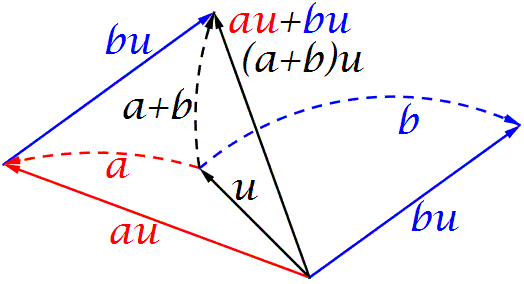
\includegraphics[width=0.5\textwidth]{imagenes/imagenes01/T01IM01.png}
		%\caption{Los dos problemas clásicos del cálculo: trazado de tangentes y áreas bajo curvas.}
	%\end{figure}
		



%\rotatebox{180}{\leftline{\textcolor{gris}{tararí}}}.